\chapter{Design and Implementation}
\label{cha:design}

This chapter presents the design and implementation of our system, focusing on the integration of the various components and the overall architecture. The system is designed to be modular, scalable, and extensible, enabling the integration of additional components as needed.

\section{Assumptions}

In this section we present the assumptions made during the design and implementation of the system. 

\subsection{Workload definition}
In this work, workloads has been modeled as \textbf{Virtual Machines (VMs)}, representing the \textbf{primary use case} considered during the system's initial design phase. 
It is possible to define as interrupible workloads, those workloads that can be stopped and restarted without losing the work done. 
For this first iteration of the system only \textbf{non-interruptible workloads} are considered.
This choice was driven by the fact the Virtual Machines are both a common and widely used cloud and one of the simplest cloud resources to provision and therefore ideal for the first iteration of the system.
Having said that, for the purpose of this work, a formalization can be done.

A VM is defined as a tuple:

\[
\text{VM} = (\text{MinCPU}, \text{MinRAM}, D, DL, ML)
\]

where:
\begin{itemize}[itemsep=0.2pt, topsep=1pt]
    \item \( \text{MinCPU} \) is the minimum number of virtual CPUs required.
    \item \( \text{MinRAM} \) is the minimum RAM required (in GB).
    \item \( D \) is the duration for which the VM must run to complete its processing task \( P \) (in hours).
    \item \( DL \) is the deadline timestamp by which the VM must complete execution.
    \item \( ML \) is the maximum allowed latency in milliseconds. If latency is not a constraint, then a high value can be set (e.g., \( ML = 2000 \)). \\
\end{itemize}

This VM can be scheduled on any Public Cloud Provider since we are interested in a multi-cloud system where the cloud can be effectively seen as a commodity. 
Alternatively, a subset of \textbf{eligible Public Cloud Providers} can be set at runtime by the user.
We will refer to \textbf{general-purpose VMs} and not specialized ones like GPU instances or high-performance computing instances. \\

As an example, we can define a VM with the following specifications:

\[
\text{VM}_{\text{example}} = (4, 4, 2, \texttt{"2025-03-20T23:59:59Z"}, 100)
\]


where:
\begin{itemize}[itemsep=0.2pt, topsep=1pt]
    \item \( \text{MinCPU} = 4 \) vCPUs
    \item \( \text{MinRAM} = 4 \) GB
    \item \( D = 1 \) hour
    \item \( DL = \texttt{"2025-03-20T23:59:59Z"} \) (i.e., the processing task \( P \) inside the VM must complete before this timestamp) \\
\end{itemize}

The system is designed to be cloud-agnostic, however for the purpose of this work, the system is currently configured to support three major cloud providers: \textbf{Microsoft Azure}, \textbf{Google Cloud Platform (GCP)}, and \textbf{Amazon Web Services (AWS)}.

\subsection{System limitations}

A limitation of our general approach is that only resources supported by the cloud provider’s Kubernetes operator can be provisioned in a 
seamless way.
Not all cloud resources available in a provider’s portfolio are guaranteed to have corresponding Kubernetes Custom Resources (CRs). This introduces certain constraints:

\begin{itemize}[itemsep=0.2pt, topsep=1pt]
  \item[$\bullet$] Limited resource availability: if a specific resource type (e.g., a GPU-accelerated instance or a database service) is not supported by the cloud provider Operator, it cannot be provisioned using the current system.
  \item[$\bullet$] Dependence on Operator updates: cloud providers may extend or modify the set of resources supported by their Kubernetes operators over time.
  \item[$\bullet$] Vendor-specific implementations: for the same class of resources (e.g., virtual machines), the structure and fields of the CRs may vary a lot between cloud providers.
\end{itemize}

Despite these constraints, the system architecture remains highly adaptable, and future enhancements could incorporate additional or alternative provisioning mechanisms. 
An example of an alternative implementation could be the \textbf{direct API interactions} with cloud providers to bypass operator limitations. As a matter of fact, usually cloud provider Operators are leveraging these APIs under the hood to interact with the cloud provider’s services.
Another approach could involve the development of custom operators or controllers to manage specific resource types not supported by existing operators. 

[KRATEO custom REST operator description]

\section{System Architecture}
\label{sec:system_architecture}

The following table provides an overview of the main components of the system and their respective functions.

\begin{table}[H]
  \centering
  \renewcommand{\arraystretch}{1.3} % Adjust row height for readability
  \begin{tabularx}{\textwidth}{| l | X |} % 'X' makes the second column auto-wrap
    \hline
    \textbf{Component} & \textbf{Function} \\
    \hline
    Krateo PlatformOps & Provides an abstraction layer for infrastructure orchestration, enabling declarative resource management and integration with cloud providers with templates. \\
    \hline
    Cloud Providers Kubernetes Operators & Manages the provisioning and reconciliation of cloud resources within Kubernetes, ensuring the actual state matches the desired state. \\
    \hline
    Kubernetes Mutating Webhook Configuration & Intercepts and modifies API requests before they are persisted, allowing dynamic configuration adjustments with policy enforcement. \\
    \hline
    OPA Server & Evaluates policy decisions based on defined constraints and input data from Kubernetes API requests through the webhook configuration. \\
    \hline
    OPA Policies and Data & Define the rules and contextual information used by OPA to make policy decisions, namely scheduling information \\
    \hline
    GreenOps Scheduler & Determines the optimal scheduling region and scheduling time for VMs, acting as an external data source for OPA policies. \\
    \hline
    MLflow & Allows the tracking, logging, versioning and storing of machine learning experiments for reproducibility and model lifecycle management. \\
    \hline
    KServe & Provides scalable and Kubernetes-native model serving capabilities, enabling deployment of machine learning models for inference. \\
    \hline
  \end{tabularx}
  \caption{Main components of the system and their respective functions.}
  \label{tab:system_components}
\end{table}

All the components listed in the above table must be deployed inside a Kubernetes cluster. The only exception are the OPA Policies and data which lies outside the cluster as described in section \ref{sec:opa_bundles}.

\section{Krateo PlatformOps integration}

Krateo PlatformOps is utilized in this system for \textbf{multi-cloud resource management}, allowing for the declarative orchestration of cloud resources across different cloud providers leveragin Kubernetes as a control plane. 
This section highlights the differences between two approaches for resource synchronization:
\begin{itemize}[itemsep=0.2pt, topsep=1pt]
  \item[$\bullet$] The \textbf{Custom Kubernetes ``Synchronization Operator"} approach
  \item[$\bullet$] The \textbf{Krateo PlatformOps} approach
\end{itemize}

It is deemed interesting to describe both approaches in order to identify the several trade-offs between implementing a custom synchronization operator and leveraging a template-based abstraction for cloud resource provisioning.

\subsection{Resource management: the Custom Kubernetes ``Synchronization Operator" approach}

When dealing with multi-cloud workloads with Kubernetes as a control plane, a synchronization and mapping mechanism (broker) is required to bridge the gap between:
\begin{itemize}[itemsep=0.2pt, topsep=1pt]
  \item[$\bullet$] \textbf{Generic Kubernetes Custom Resources}, which represent generic provider-agnostic workloads.
  \item[$\bullet$] \textbf{Cloud provider-specific Custom Resources}, which correspond to the actual cloud resources provisioned through the respective Kubernetes operators provided by Azure, AWS or GCP (in our case).
\end{itemize}

A custom Kubernetes Operator would be responsible for the mapping and synchronization of the above resource types. This approach is based on the principle of \textbf{Continuous Reconciliation}, where the operator continuously monitors and adjusts the system to maintain consistency between the desired and actual states.
Candidate solutions for the development of the K8s Operator includes: Operator SDK, Kubebuilder, or writing the operator from scratch using the Kubernetes client libraries. For the purpose of this work, Kubebuilder was used to develop a Proof of Concept (PoC) for the custom synchronization operator.

\subsubsection{Responsibilities of the Custom Operator}

In our specific case, the operator should continuously watch the generic CRs in the Kubernetes cluster to check if critical scheduling fields have been set:
\begin{itemize}[itemsep=0.2pt, topsep=1pt]
  \item[$\bullet$] \textbf{schedulingRegion}: Defines where the workload should be placed.
  \item[$\bullet$] \textbf{schedulingTime}: Specifies when the workload should be deployed.
\end{itemize}

These fields, if set, indicate a geographical placement and timing for the workload have been determined by the GreenOps Scheduler.
If these fields are not yet present, the operator must wait for scheduling decisions before proceeding.
Therefore, inside its Reconcile() loop, the operator should:
\begin{enumerate}[itemsep=0.2pt, topsep=1pt]
  \item Continuously check if scheduling fields (schedulingRegion, schedulingTime) are set.
  \item Trigger the creation of the provider-specific resource when the schedulingTime is approaching.
  \item Track the provisioning status by marking the generic CR with a field indicating that the cloud-specific resource has been created.
\end{enumerate}

\subsubsection{Post-Creation Considerations}

Once the cloud provider-specific resource is created, two main questions arise:
\begin{itemize}[itemsep=0.2pt, topsep=1pt]
  \item[$\bullet$] What happens if the provider-specific CR is modified manually?
  \item[$\bullet$] What happens if the VM configuration is modified directly on the cloud provider (outside Kubernetes)?
\end{itemize}

Related to the first question, an example scenario could be: changing the VM instance type (VM size) inside the Kubernetes cluster. In this case, the operator needs to decide whether to revert unauthorized changes or allow them and update the generic CR accordingly.
For the second question, an example could be: changing the VM size directly on the cloud provider’s console. In this case, the operator should detect the drift and update the generic CR to reflect the external changes.

\subsubsection{Resource linking}

A mechanism must be in place to link the generic CR to the cloud provider-specific CR. Possible approaches include:
\begin{itemize}[itemsep=0.2pt, topsep=1pt]
  \item[$\bullet$] UUID-based linking: A universally unique identifier ensuring each resource is mapped correctly.
  \item[$\bullet$] Kubernetes Object Metadata (ObjectMetadata.Name \& ObjectMetadata.Namespace): This approach may be preferable within a single Kubernetes cluster, avoiding the need for an external ID system.
\end{itemize}

\subsubsection{Termination Logic}

The operator must handle the deletion of cloud resources correctly in a variety of scenarios:
\begin{itemize}[itemsep=0.2pt, topsep=1pt]
  \item[$\bullet$] When the provider-specific CR is deleted from Kubernetes, the corresponding cloud resource is de-provisioned and the custom operator should ensure the deletion process is handled gracefully, avoiding orphaned generic CRs.
  \item[$\bullet$] If the provider-specific CR is deleted directly on the cloud provider, the operator should detect the change and update the generic CR accordingly.
  \item[$\bullet$] In the event of a generic CR deletion, the custom operator should ensure the provider specific resource is removed, troggering a deletion process on the cloud provider side (de-provisioning).
\end{itemize}

\subsubsection{Managing cloud provider-specific fields}
Each cloud provider has unique resource configurations and constraints that must be managed.
Some differences are purely syntactic (e.g., AWS uses instanceType, whereas Azure uses vmSize).
Others require additional provider-specific metadata (e.g., Azure requires a resourceGroup field which represent a logical container for resources in Azure).
A custom synchronization operator must encode this logic explicitly, making it more complex to maintain especially when supporting several cloud providers.

\subsubsection{Limitations of a Custom ``Synchronization Operator''}
Another major challenge with a custom synchronization operator is that some cloud providers do not support time scheduling metadata within their Custom Resources. In particular, no cloud operator among the ones we used for the system (AWS, Azure, GCP) provides a dedicated field for scheduling time.
This means that the Kubernetes operator itself must handle time scheduling logic, delaying CR creation until the scheduled time.
If the operator, upon the creation of a generic CR, immediately creates the cloud-provider specific CR (without a ``waiting logic''), the cloud provider Operator will trigger and provision the VM immediately, ignoring scheduling constraints.
Due to these limitations and complexities, we explored and leveraged an \textbf{alternative template-driven approach} using Krateo PlatformOps, described in the next section.

\begin{figure}[htb]
  \centering
  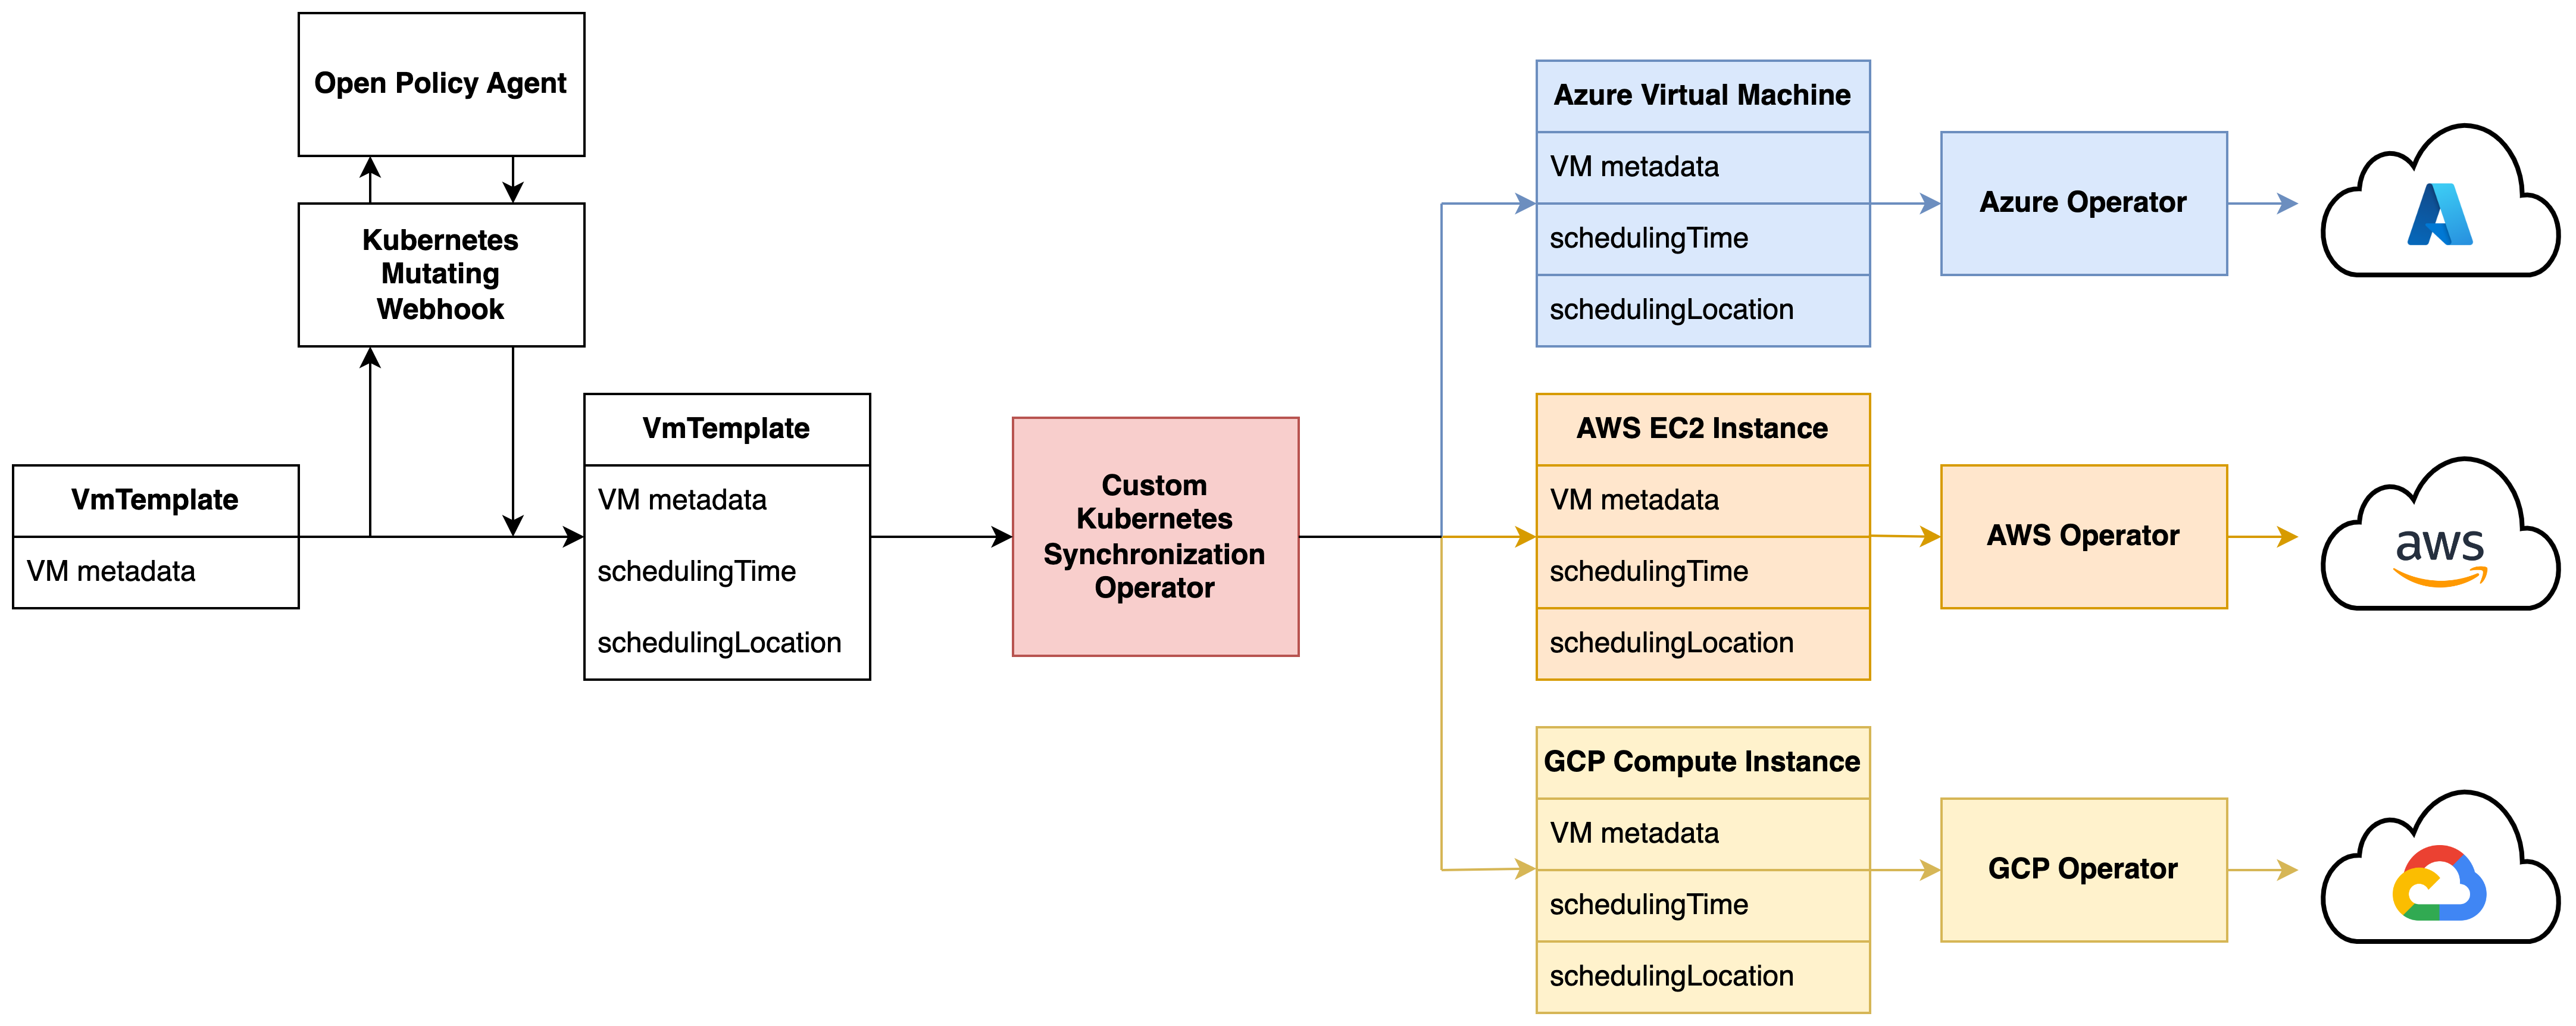
\includegraphics[width=1\linewidth]{images/k8s_operator.png}
  \caption{Multi-cloud resource management with Custom Kubernetes ``Synchronization Operator'' approach}
  \label{fig:k8s_operator}
\end{figure}

\subsection{Resource management: the Krateo approach}

\begin{figure}[htb]
  \centering
  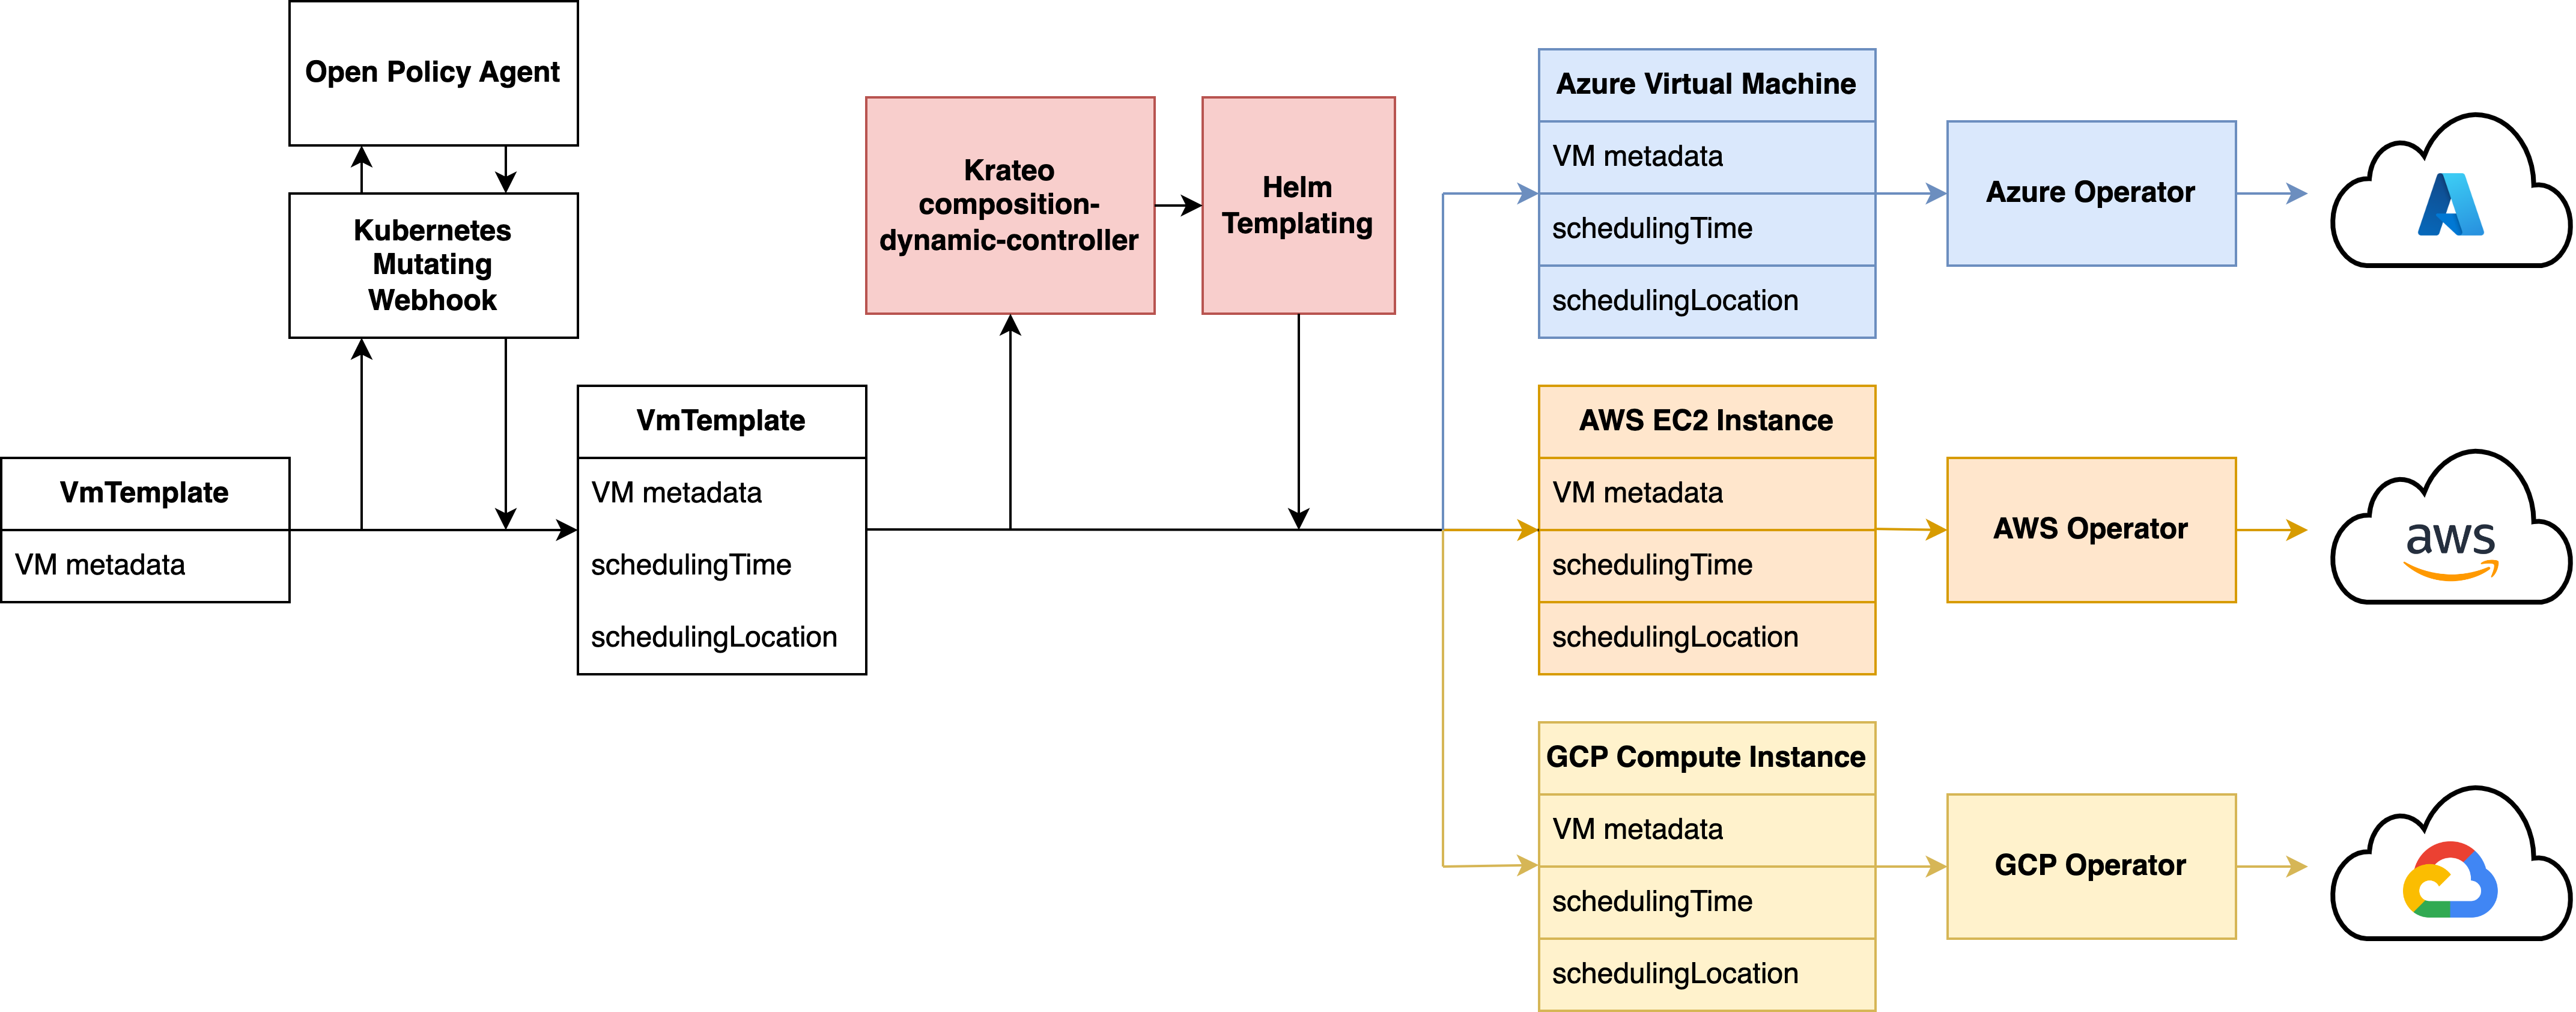
\includegraphics[width=1\linewidth]{images/krateo.png}
  \caption{Multi-cloud resource management with Krateo PlatformOps approach}
  \label{fig:krateo}
\end{figure}


krateo already described in section \ref{xyz}

Self-service platform for multi-cloud native resources

(generic VM mapped thanks to Krateo components, what is the added value)

generic workload resource definition
how to define it


\begin{lstlisting}[language=yaml, caption={values.yaml}, label={lst:values.yaml}, float=htpb]
# @param {string} vmName Name of the VM
vmName: test-vm

# @param {integer} cpu  Number of CPU cores
cpu: 1

# @param {integer} memory Number of GB of RAM
memory: 2

# @param {string} [schedulingTime] Scheduling Time for the VM
schedulingTime: 2025-05-05T00:00:00Z

# @param {string} [schedulingLocation] Scheduling Location for the VM
schedulingLocation: italynorth

# @param {string} duration Duration of the Workload
duration: 3h

# @param {string} deadline Deadline of the Workload
deadline: 2025-12-31T10:00:00Z

# @param {integer} maxLatency Maximum Latency of the Workload
maxLatency: 100
\end{lstlisting}


\lstset{style=jsonstyle}
\begin{lstlisting}[caption={values.schema.json}]
{
  "type": "object",
  "$schema": "http://json-schema.org/draft-07/schema",
  "required": [
    "vmName",
    "cpu",
    "memory",
    "duration",
    "deadline",
    "maxLatency"
  ],
  "properties": {
    "vmName": {
      "type": [
        "string"
      ],
      "description": "Name of the VM",
      "default": "test-vm"
    },
    "cpu": {
      "type": [
        "integer"
      ],
      "description": "Number of CPU cores",
      "default": "1"
    },
    "memory": {
      "type": [
        "integer"
      ],
      "description": "Number of GB of RAM",
      "default": "2"
    },
    "schedulingTime": {
      "type": [
        "string"
      ],
      "description": "Scheduling Time for the VM",
      "default": "2025-05-05T00:00:00Z"
    },
    "schedulingLocation": {
      "type": [
        "string"
      ],
      "description": "Scheduling Location for the VM",
      "default": "italynorth"
    },
    "duration": {
      "type": [
        "string"
      ],
      "description": "Duration of the Workload",
      "default": "3h"
    },
    "deadline": {
      "type": [
        "string"
      ],
      "description": "Deadline of the Workload",
      "default": "2025-12-31T10:00:00Z"
    },
    "maxLatency": {
      "type": [
        "integer"
      ],
      "description": "Maximum Latency of the Workload",
      "default": "100"
    }
  }
}
  
\end{lstlisting}


Helm template engine (how to map to cloud provider specific resources, why is better)


Multi-cloud VMs list and mapping
We need to know which VMs (instance types) are actually available on Azure, AWS, GCP.
What to actually use to fetch the list and where to store it
How frequent the elements changes and how to update the list (this is done with policy updates (updates to contextual data))
How to match generic workload to candidate VMs instance types (that adhere to the generic workload specs), what is the mapping logic.
For example:
Requested VM (generic): (2 vCPU, 16 GiB)
Chosen VM instance: Azure Standard E2as v4
What are the steps of the process to identify the correct VM instance?

Use Cloud Providers API / CLI and store the records in a local DB. Regular scheduled updates.
For our PoC we could maybe use a small subset of all the available instance types.

Current approach:
Map (CPU, RAM) => InstanceType

This mapping is done through Helm templating when creating 

compostion definition


krateo cdc
The composition-dynamic-controller is an operator that is instantiated by the core-provider to manage the Custom Resources whose Custom Resource Definition is generated by the core-provider.

\section{Kubernetes Mutating Webhook Configuration}

\subsection{Kubernetes Admission Control}

In the context of \textbf{Kubernetes Admission Control}, in addition to standard, compiled-in admission plugins, Kubernetes supports the use of additional admission plugins that are effectively extensions of the system and run as \textbf{webhooks} configured at runtime \cite{kubernetes_dynamic_admission_control}. This means that the admission control logic can be extended dynamically without the need to recompile the Kubernetes API server or other Kubernetes components. Changes are applied at runtime to the running Kubernetes cluster, making the system more flexible and adaptable.











These plugins can be used to enforce custom policies and perform additional validation and mutation of Kubernetes objects before they are persisted in the cluster.

K8s mutating webhook is used to modify K8s custom resources with the data from policies. 
The K8s mutating webhook intercepts the CREATE or UPDATE API request, asks about policies (with also scheduling decision) and mutates the resource.

we can distinguish between two types of webhooks: validating and mutating.

we can distinguish two entities semantically different: the webhook configuration and the actual webhook /server which perform mutation or validation

it could be a server that you need to implement to perform your own custum mutation or validation logic
it could be a service ready to use out of the box like OPA server

\begin{figure}[htb]
  \centering
  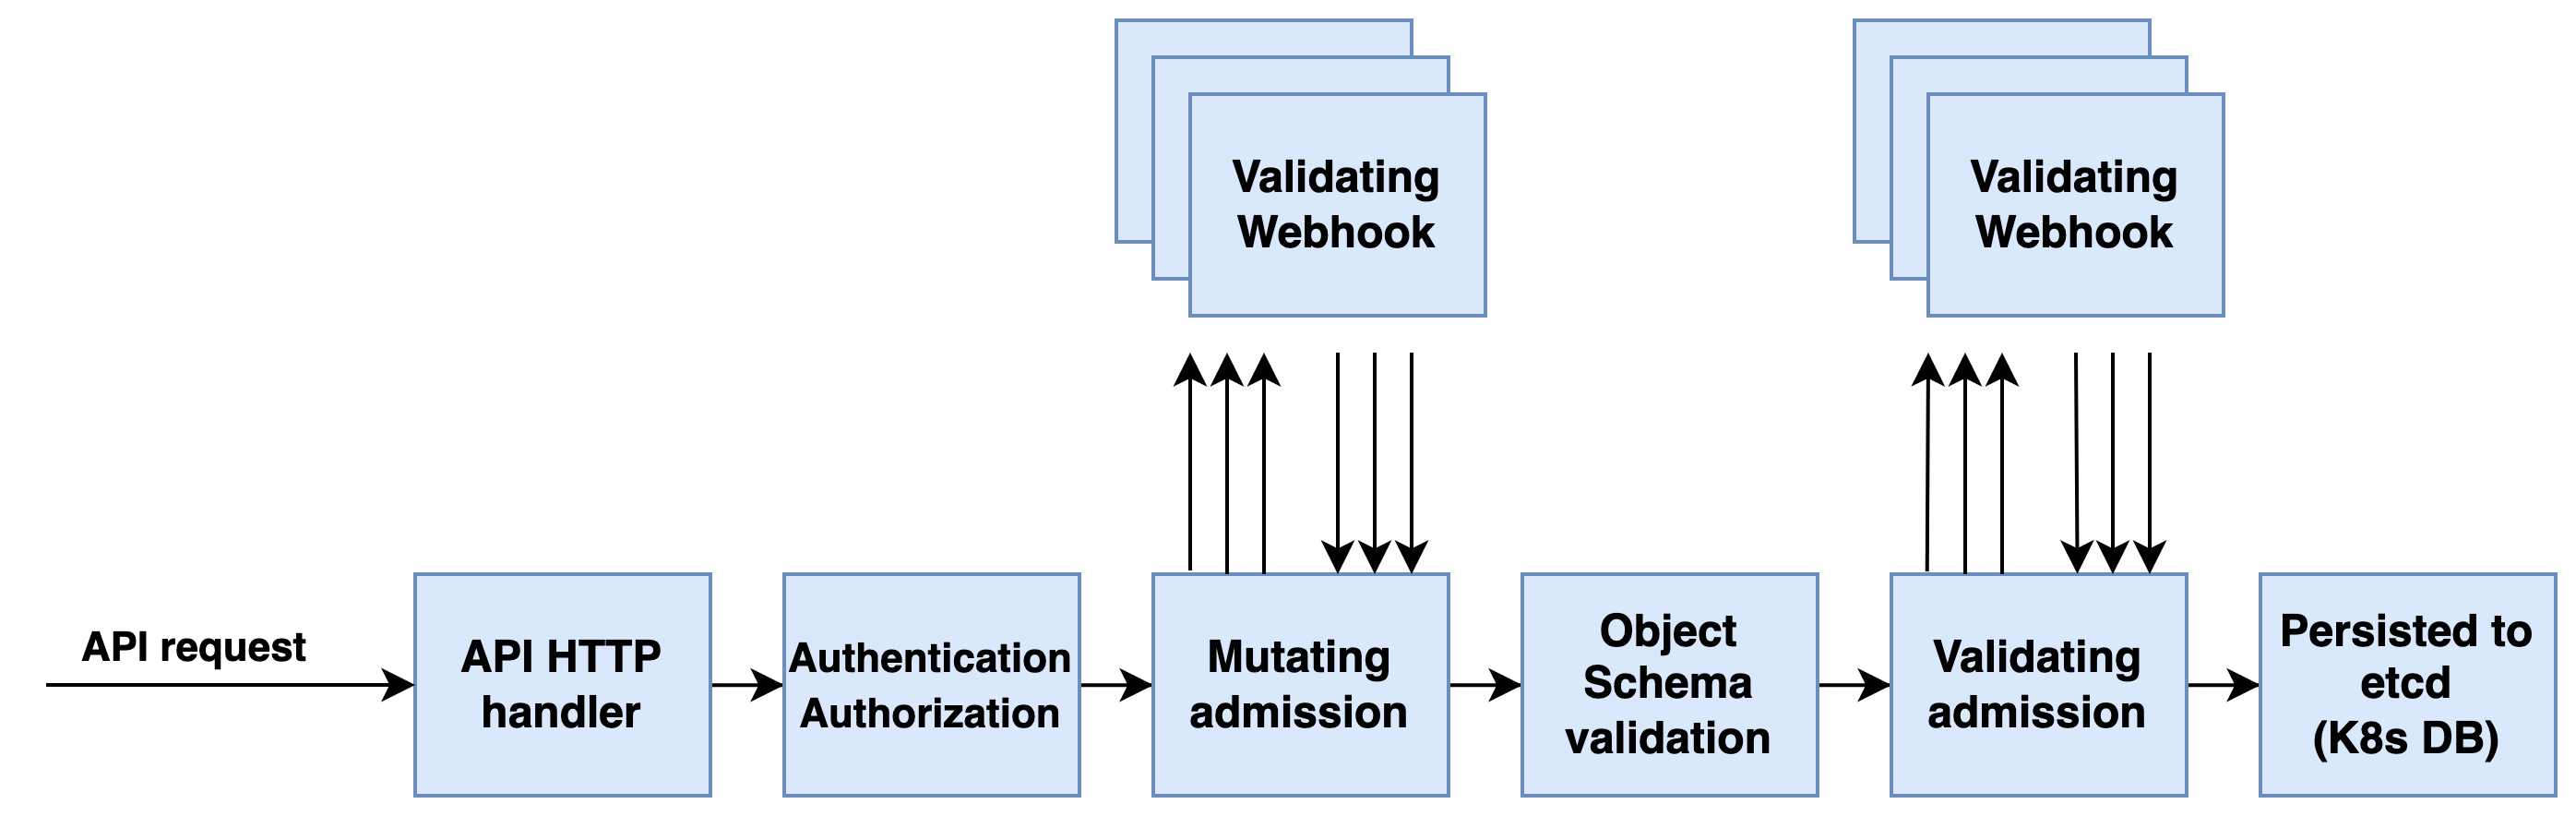
\includegraphics[width=1\linewidth]{images/k8s_admission.png}
  \caption{Kubernetes Admission Control}
  \label{fig:k8s_admission_control}
\end{figure}


service can be either a deployment with the related service inside the cluster like seen in the image \ref{fig:k8s_webhook_example}

or can be deployed outside the cluster

Figure \ref{fig:k8s_webhook_example} shows an example of a Kubernetes Mutating Webhook. The webhook server is deployed as a Kubernetes Deployment (with 1 Pod), with a corresponding Service to expose it within the cluster. The webhook server is responsible for receiving The AdmissionReview Request, applying custom logic, and returning an AdmissionReview Response to the Kubernetes API server describing the mutation to be applied to the resource.
The custom logic in this simple example is just to add a label "mutated: true" to the resource.

\begin{figure}[htb]
  \centering
  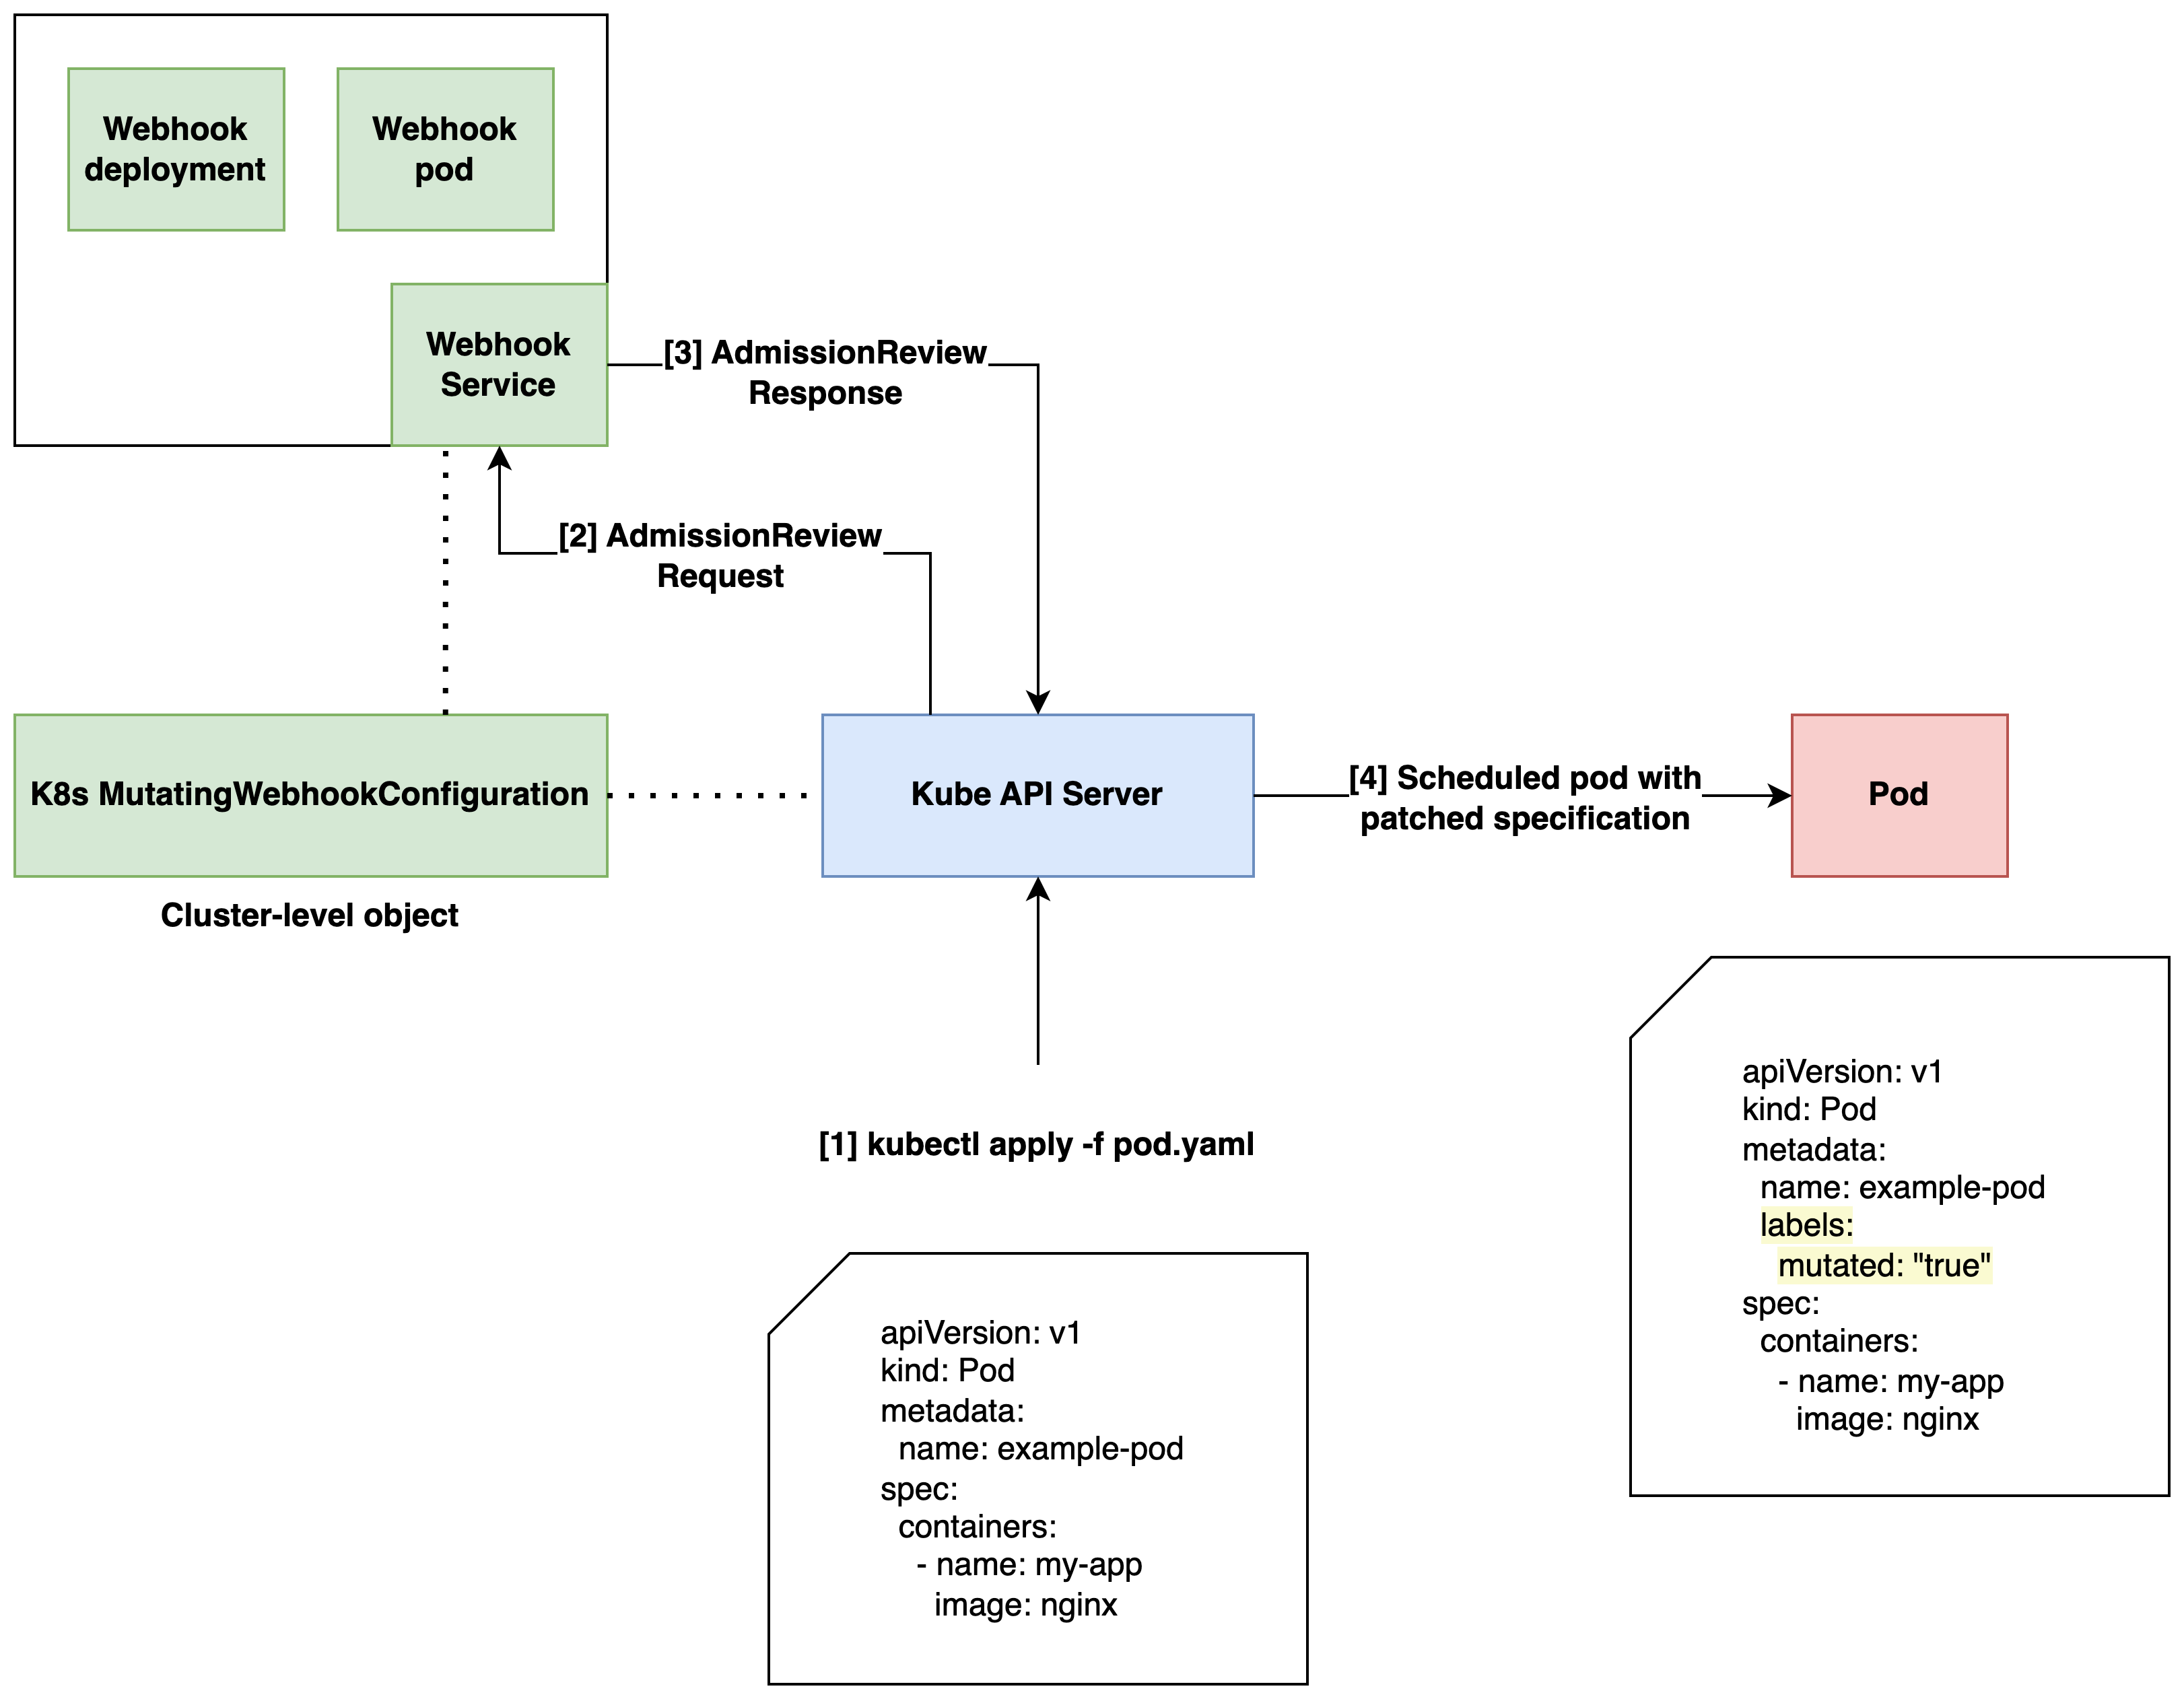
\includegraphics[width=1\linewidth]{images/k8s_webhook_example.png}
  \caption{Kubernetes Mutating Webhook example \cite{kubernetes_mutating_webhook_example}}
  \label{fig:k8s_webhook_example}
\end{figure}

\section{Multi-Cloud Integration through Kubernetes Operators}

The integration of operators from different cloud providers has enabled the development of an effective \textbf{multi-cloud system}, allowing seamless orchestration and provisioning of cloud resources across various cloud platforms. Namely, the system leverages Kubernetes operators from \textbf{Microsoft Azure}, \textbf{Google Cloud Platform (GCP)}, and \textbf{Amazon Web Services (AWS)}.

\subsection{Role of Kubernetes Operators}

Kubernetes operators work on the principle of Continuous Reconciliation, ensuring, in this case, that the desired state of the system, as defined by users, aligns with the actual state of provisioned cloud resources. In particular, Operators act as controllers that monitor, adjust, and manage external cloud resources within a Kubernetes-native environment. Inside the K8s lie the representation of the cloud resources, which are managed by the operators.
Key characteristics of operators include:
\begin{itemize}[itemsep=0.2pt, topsep=1pt]
  \item[$\bullet$] Managing external cloud resources within a Kubernetes cluster, providing a \textbf{unified interface} for multi-cloud deployments.
  \item[$\bullet$] Maintaining a \textbf{real-time representation} of provisioned cloud resources within Kubernetes.
  \item[$\bullet$] Using Custom Resources (CRs) to define cloud-specific resources in a \textbf{declarative} manner.
\end{itemize}

\subsection{Strategic Shift: From Custom Operator to Krateo Core Provider}

In our approach, we opted to replace a custom Kubernetes operator (``Synchronization Operator''), originally designed to handle the \textbf{mapping} from generic to cloud-specific resources, with \textbf{Krateo Core Provider}. This decision was motivated by the need for greater flexibility and maintainability in defining multi-cloud infrastructure components. As a matter of fact, the custom operator was originally designed to handle only virtual machines (VMs) mappings and extensions to support additional cloud resources would have required significant code changes and maintenance overhead for each additional resource type added.

Therefore instead of embedding business logic directly within a custom Kubernetes operator, in the current system implementation, we leverage the capabilities of \textbf{Helm templating} to dynamically generate cloud-provider-specific resources. More precisely, another Krateo component, the \textbf{Krateo composition-dynamic-controller} is leveraging Helm templating under the hood to generate Kubernetes resources starting from helm templates.
This approach, further described in the following sections, offers several advantages:

Simplified resource management:  Helm enables a standardized way define resources without maintaining complex operator logic.
Greater extensibility:  By externalizing the logic from the operator, future modifications and integrations with additional cloud providers become easier.
Reduced maintenance overhead: Operators typically require constant updates and refinements, while Helm-based resource generation minimizes the need for frequent code changes.

It must be noted that different cloud provider adopts different design choices for their Kubernetes operators and more in general for their overall infrastructure management. Therefore, for the creation of logically similar resources, like a virtual machine, the structure and the field of the resources can be different. 
These resources typically include:
\begin{itemize}[itemsep=0.2pt, topsep=1pt]
  \item[$\bullet$] Compute resources (e.g., VM instances, virtual machine templates)
  \item[$\bullet$] Networking components (e.g., virtual networks, subnets, security groups)
  \item[$\bullet$] Storage allocations (e.g., persistent volumes, cloud disks)
  \item[$\bullet$] Access management (e.g., resource groups, roles, authentication credentials)
\end{itemize}


For the purpose of this work we defined baseline infrastructure for each cloud provider in order to have a common ground for the system to work. This baseline infrastructure is composed by the minimum set of resources needed for a VM provisioning.

each providers has its complexities and nuances

vendor lock-in.





\newpage

\subsection{Azure Kubernetes Operator}

Microsoft Azure provides a Kubernetes operator called \textbf{Azure Service Operator v2} (ASO).
Currently, ASO supports more than 150 different Azure resources.
minimum set of resources needed for vm provisioning on Azure throgh Azure service operator is is:

\begin{itemize}[itemsep=0.2pt, topsep=1pt] \item[$\bullet$] Virtual Network 
\item[$\bullet$] Virtual Network Subnet
\item[$\bullet$] Network Interface
\item[$\bullet$] Virtual Machine
\end{itemize}

\begin{figure}[H]
\centering
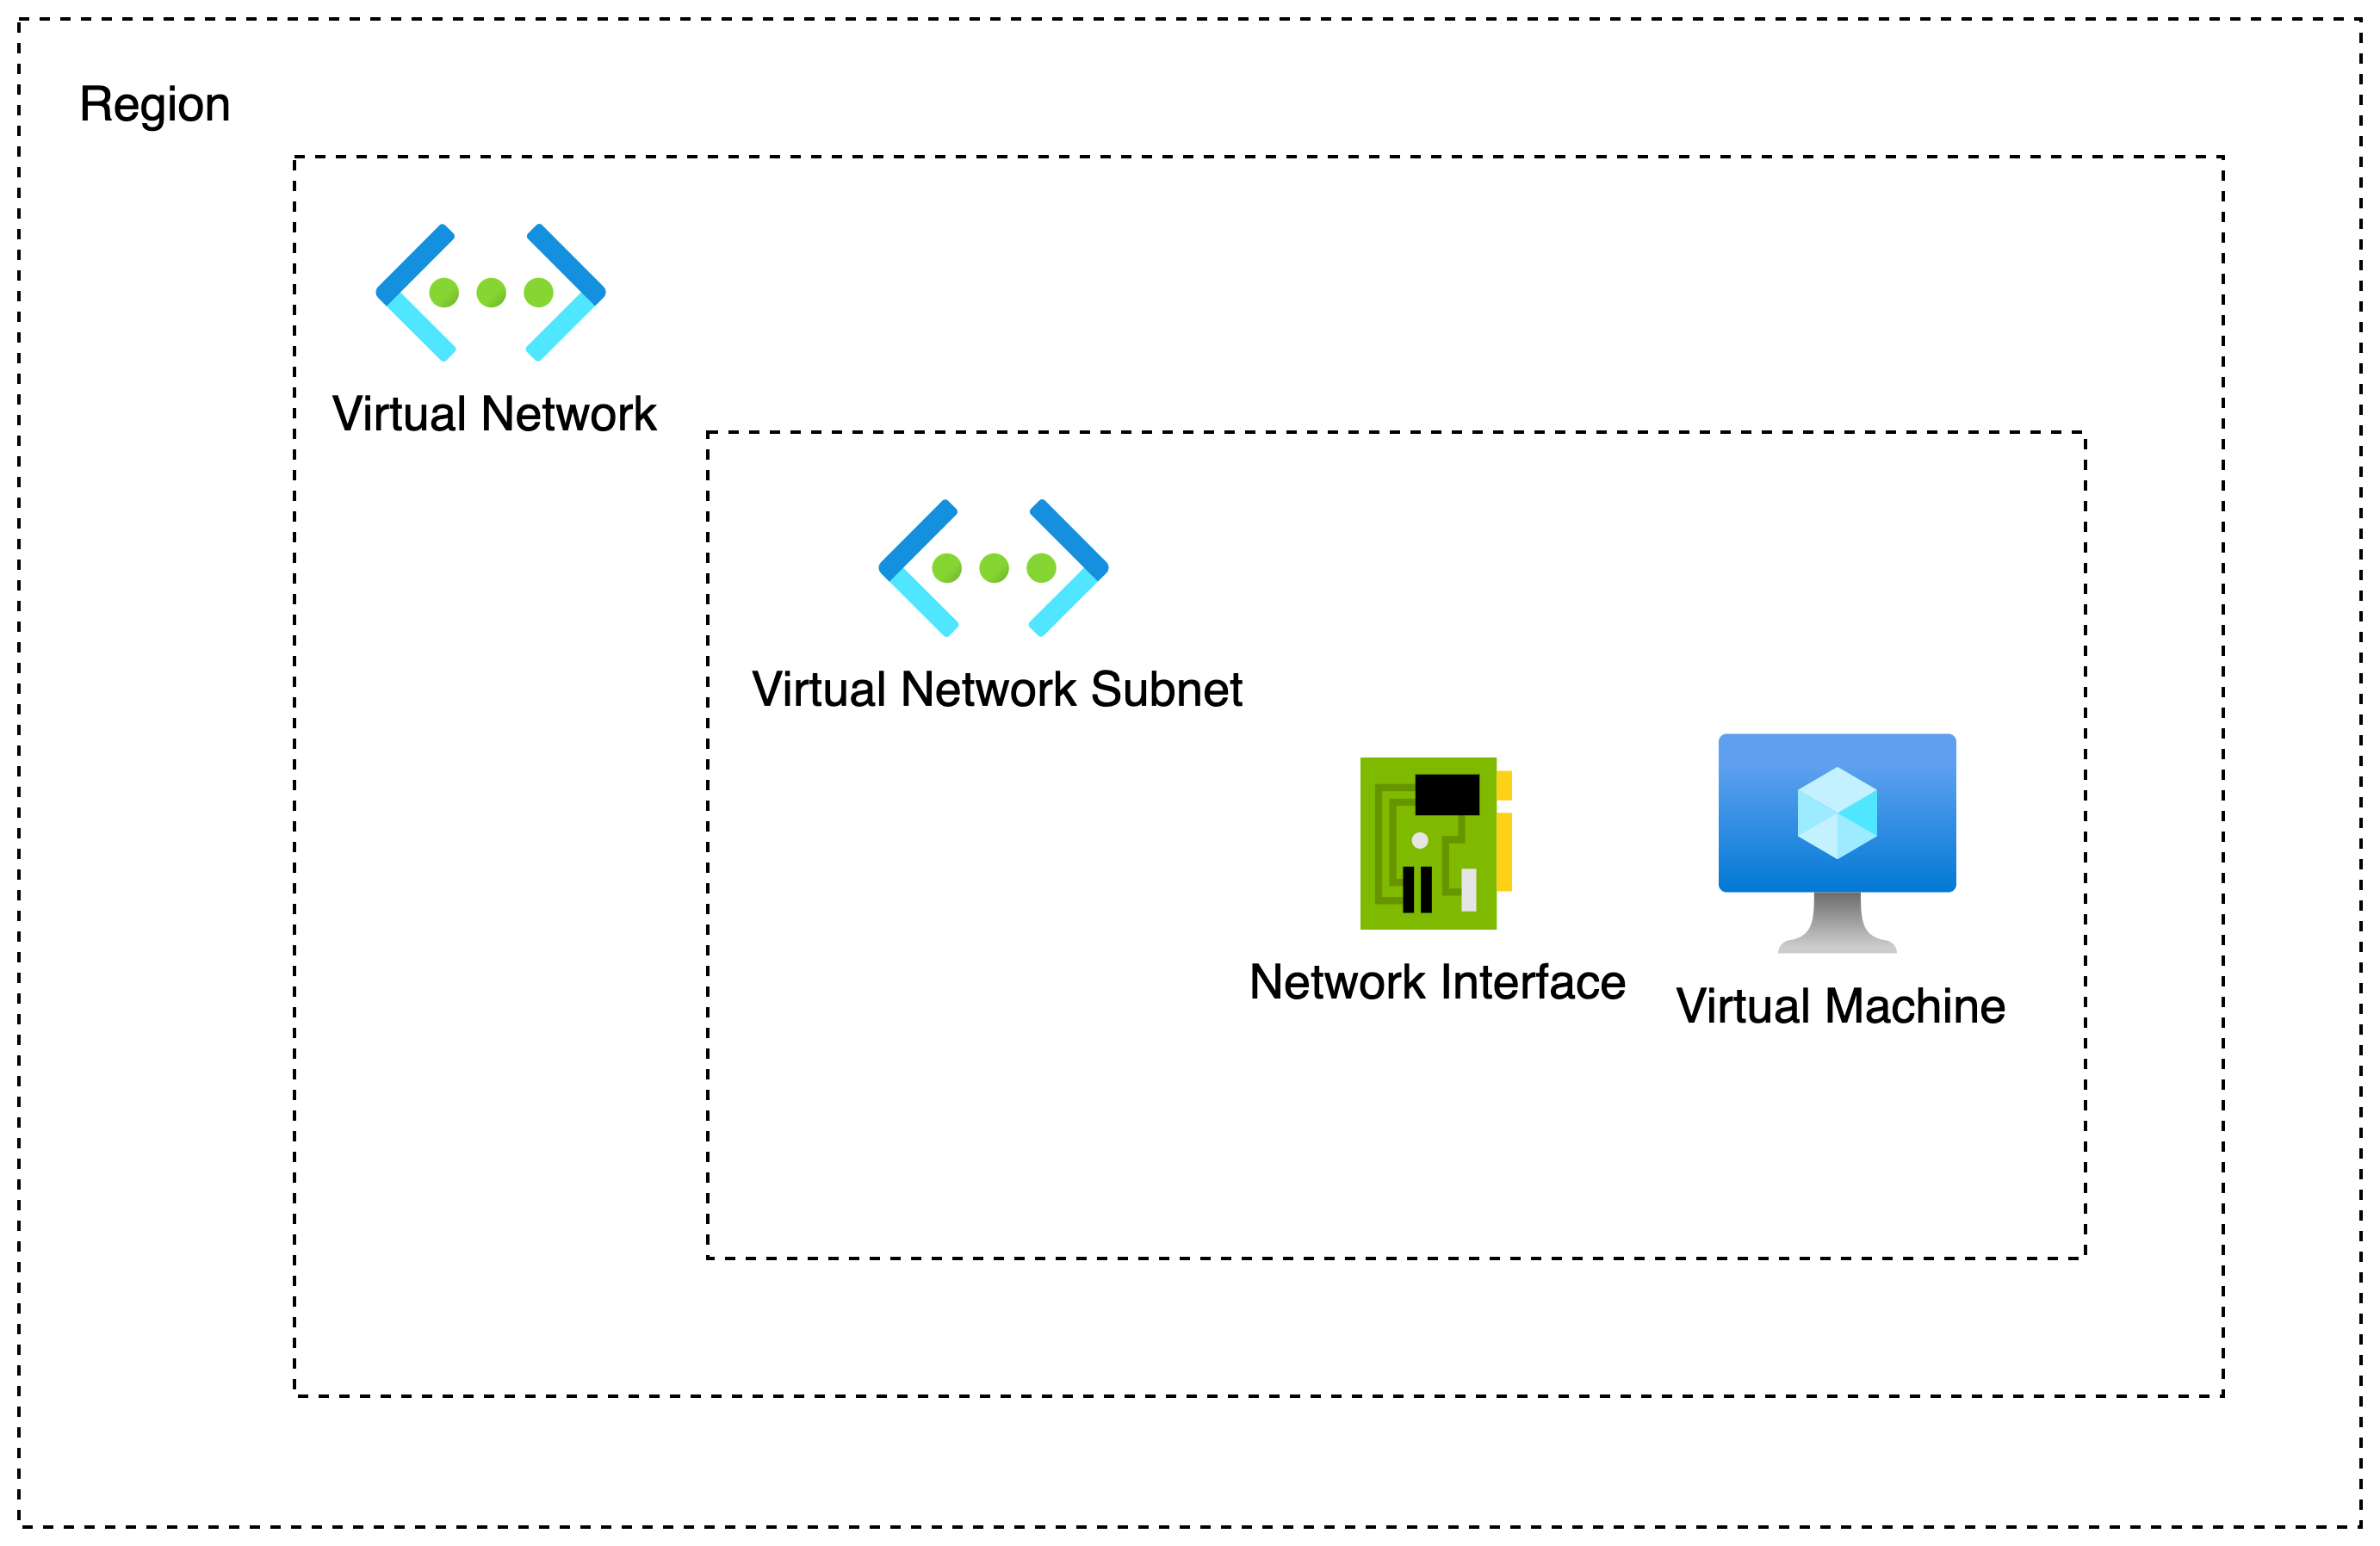
\includegraphics[width=0.75\linewidth]{images/azure.png}
\caption{Minimum set of Azure resources for VM provisioning}
\label{fig:azure}
\end{figure}






INSTANCE CR example











\subsection{GCP Operator}

minimum set of resources needed for vm deployment


\begin{figure}[H]
\centering
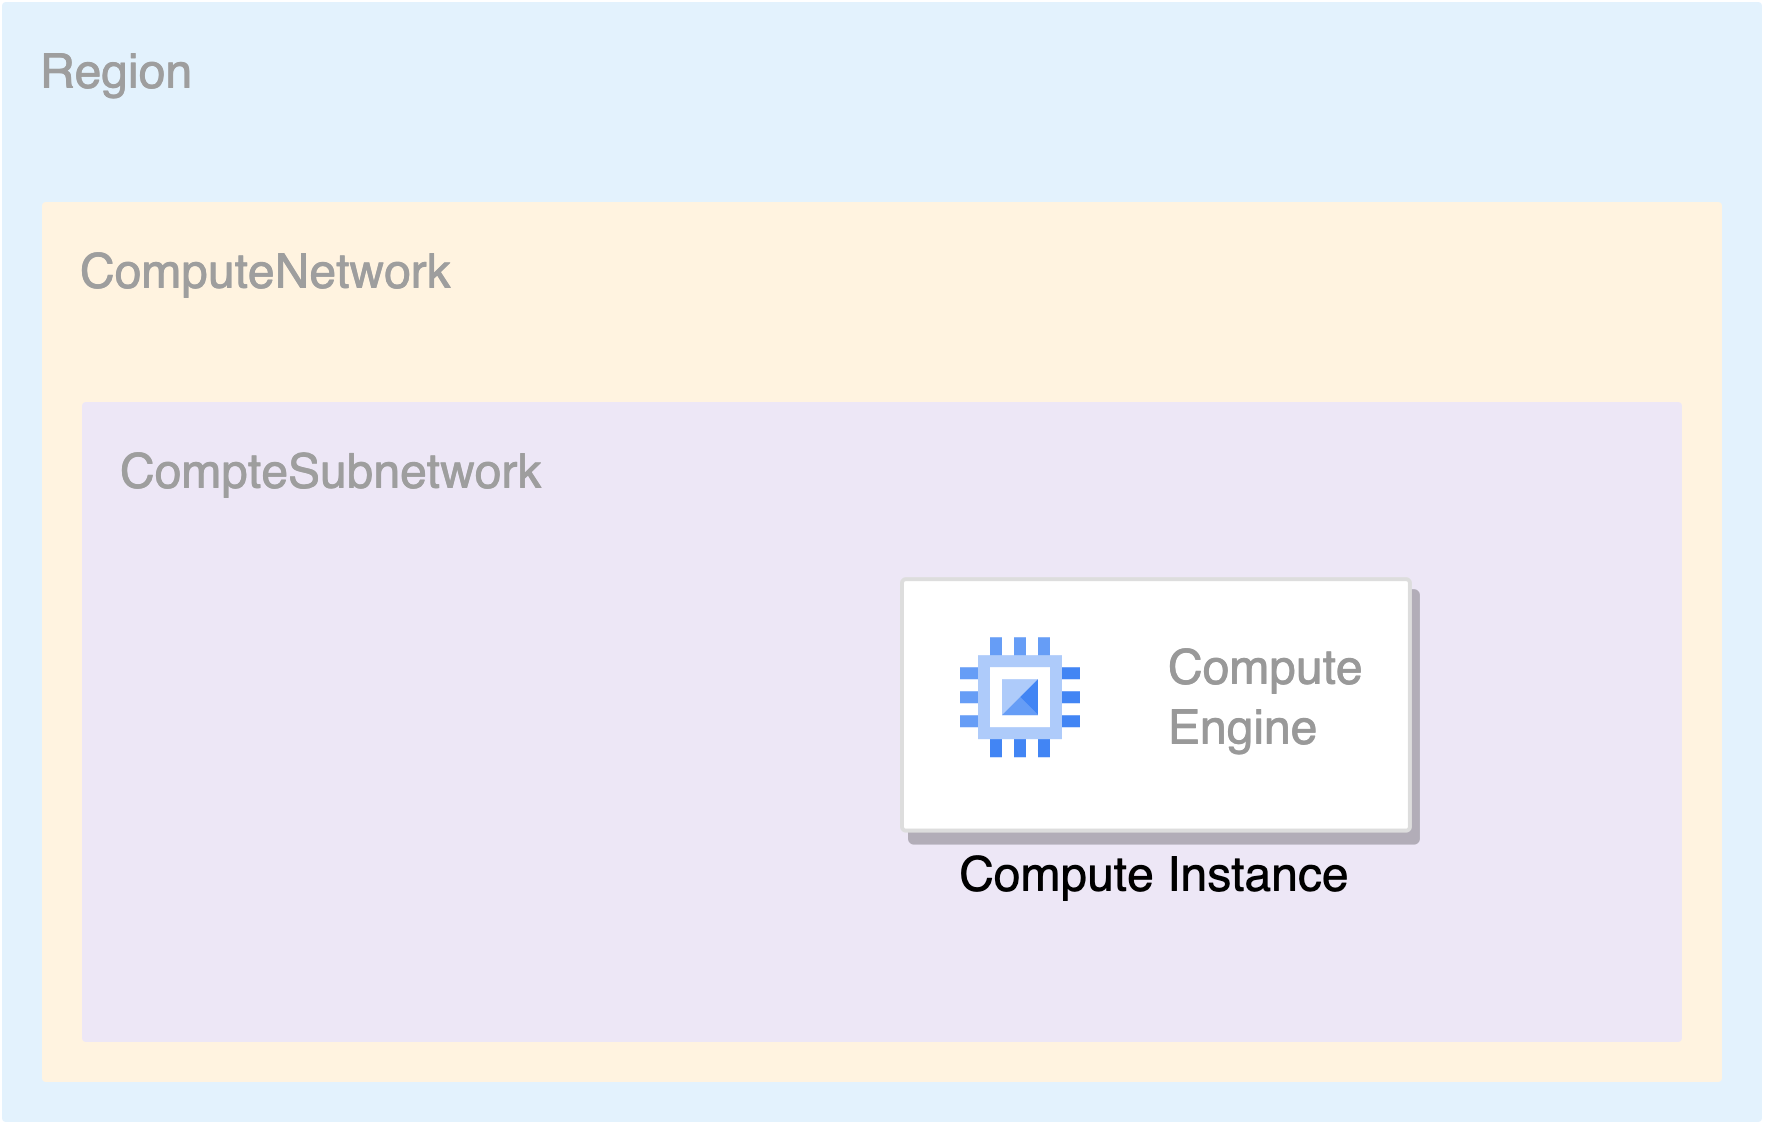
\includegraphics[width=0.75\linewidth]{images/gcp.png}
\caption{Minimum set of GCP resources for VM provisioning}
\label{fig:gcp}
\end{figure}




INSTANCE CR example

some fields are based on regions
some fields are based on zones


networkinterface is directly defined in the instance manifest,
no additional resource needed



\subsection{AWS Operator}

this is a collection of operators that are part of the AWS controllers for Kubernetes (ACK) project.

The minimum set of resources needed for vm provisioning

\begin{itemize}[itemsep=0.2pt, topsep=1pt] 
\item[$\bullet$] VPC
\item[$\bullet$] Subnet
\item[$\bullet$] EC2 Instance
\end{itemize}

\begin{figure}[H]
\centering
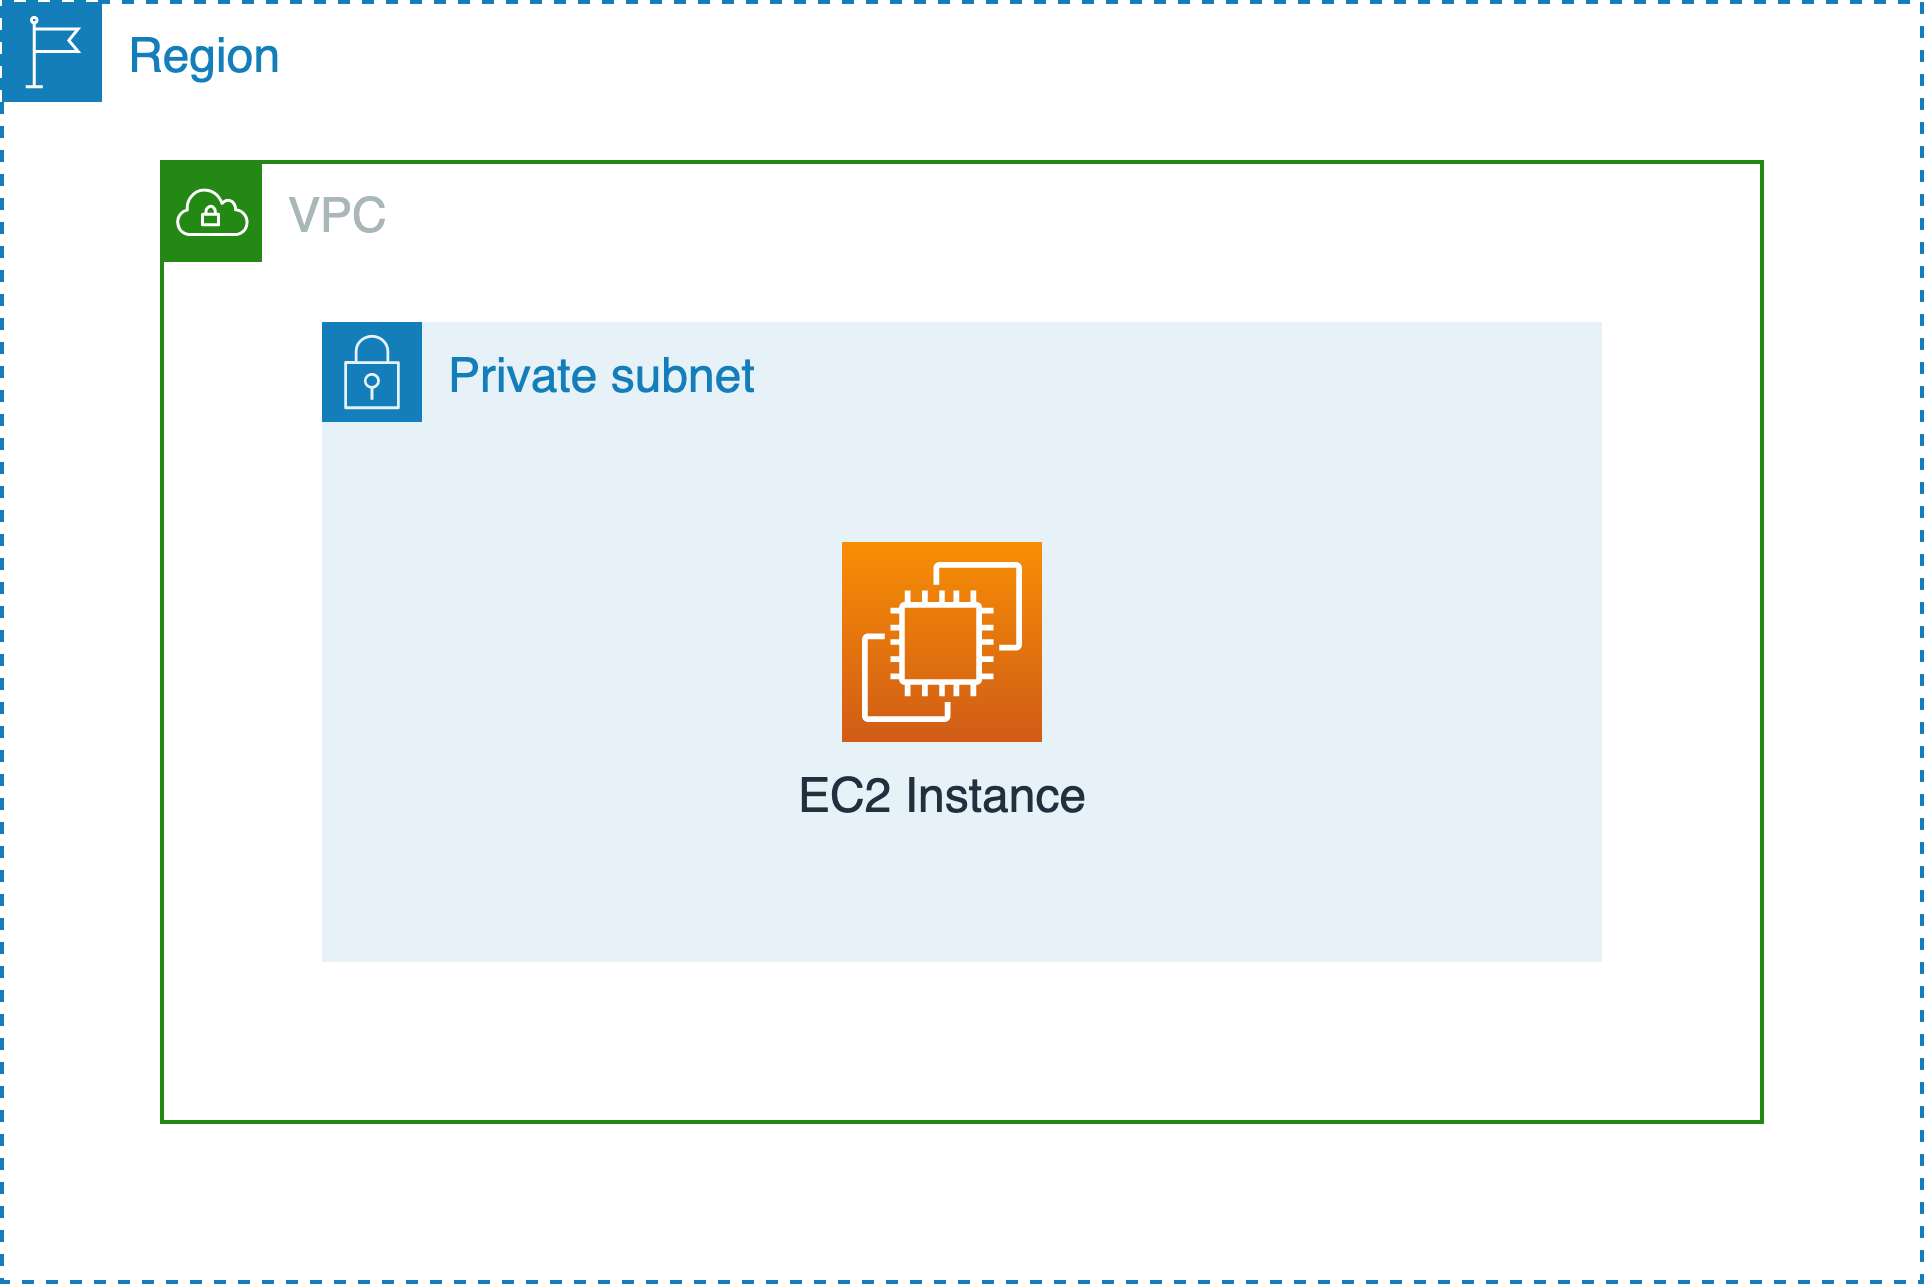
\includegraphics[width=0.75\linewidth]{images/aws.png}
\caption{Minimum set of AWS resources for VM provisioning}
\label{fig:aws}
\end{figure}

As described at the beginning of this section, the implementation approach adopted in our system ensures compatibility with diverse cloud provider design choices. Cloud providers may impose different constraints and best practices when managing Kubernetes-native resources, and the system is designed to adapt to these variations seamlessly.

One notable design choice observed with the AWS operator is the restriction on referencing some Kubernetes objects inside a Custom Resource (CR) manifest. This limitation means that developers cannot directly link a resource (e.g., a Virtual Machine) to another Kubernetes object (e.g., a Subnet) using built-in object references.

To overcome this limitation, our system leverages \textbf{Helm’s \textit{lookup function}}, which dynamically retrieves Kubernetes object details at runtime. This method allows us to fetch required parameters without directly referencing Kubernetes objects in the CR, ensuring compatibility with the AWS operator’s design constraints. The following example demonstrates how the lookup function can be used to resolve subnet IDs dynamically and inject them into the CR manifest. \\

\begin{lstlisting}[language=yaml, caption={Helm Lookup example: dynamically resolving SubnetIDs}, label={lst:helm_lookup}, float=htpb]
...
apiVersion: ec2.services.k8s.aws/v1alpha1
kind: Instance
metadata:
  name: {{ .Values.vmName }}
  namespace: {{ .Values.namespace | default "greenops" }}
...
spec:
  ...
  subnetID: {{ (lookup "ec2.services.k8s.aws/v1alpha1" "Subnet" (.Values.namespace | default "greenops") (printf "%s-subnet" .Values.vmName)).status.subnetID }}
...
\end{lstlisting}

The Helm lookup function can be used to look up resources in a running cluster and its synopsis is: ``lookup apiVersion, kind, namespace, name -> resource or resource list'' \cite{helm_lookup}.
In the listing \ref{lst:helm_lookup}, the Helm lookup function retrieves the subnetID from a Subnet Custom Resource dynamically, based on the VM name and namespace. Then, the subnetID is injected into the Instance Custom Resource manifest, ensuring that the VM is provisioned in the correct subnet.

An example by the same AWS Operator where instead a direct reference to a resource is allowed is the one illustrated in listing \ref{lst:aws_direct_reference}. \\

\begin{lstlisting}[language=yaml, caption={AWS Operator direct reference example}, label={lst:aws_direct_reference}]
...
apiVersion: ec2.services.k8s.aws/v1alpha1
kind: Subnet
metadata:
  name: {{ .Values.vmName }}-subnet
...
spec:
  vpcRef: 
    from: 
      name: {{ .Values.vmName }}-vpc
      namespace: {{ .Values.namespace | default "greenops" }}
...
\end{lstlisting}

In thr case of Listing \ref{lst:aws_direct_reference}, the Subnet Custom Resource manifest directly references in a conveneint way the VPC Custom Resource using its name and namespace since the Operator is designed to support this type of relationship. As explained before, this is determined by Operator design choices but our system is able to handle both scenarios.

\subsubsection{Provider specific configurations}

An Amazon Machine Image (AMI) is a pre-configured image that provides the necessary software environment to set up and boot an Amazon EC2 instance \cite{aws_AMIs}. In other words, AMIs serve as a blueprint for launching virtual machines (VMs) in AWS.

When launching an instance, specifying an AMI is \textbf{mandatory}. The AMI must be compatible with the chosen EC2 instance type, ensuring that the selected image supports the required hardware and software configurations.

The following attributes define an AMI:
\begin{itemize}[itemsep=0.2pt, topsep=1pt] 
  \item[$\bullet$] Region: AMIs are region-specific
  \item[$\bullet$] Operating System: Determines the base OS (e.g., Ubuntu, Windows, RHEL) installed on the AMI.
  \item[$\bullet$] Processor Architecture: e.g., x86, ARM
  \item[$\bullet$] Root Device Type: Specifies whether the AMI uses an EBS-backed volume (Elastic Block Store) or Instance Store for storage.
  \item[$\bullet$] Virtualization Type: Defines whether the AMI supports paravirtual (PV) or hardware virtual machine (HVM) instances.
\end{itemize}


For the purpose of this research, only \textbf{Ubuntu-based AMIs} have been considered for provisioning virtual machines. Official Ubuntu AMIs were collected from a dedicated Ubuntu repository.
In order to select the most suitable AMI for a given VM, the system leverages Helm template engine to dynamically select the appropriate AMI ID based on the region and other parameters specified in the VmTemplate Kubernetes Custom Resource (CR).



\newpage

\section{Open Policy Agent (OPA)}

Open Policy Agent (OPA) is an open-source general-purpose \textbf{policy engine} that enables unified policy enforcement across cloud-native environments. OPA provides a declarative language called Rego enabling a paradigm known as ``\textbf{Policy as Code}" \cite{opa_docs}.

Open Policy Agent can be integrated as a sidecar container, host-level daemon, or library to perform policy decisions for a plethora of use cases: microservices, Kubernetes admission control, CI/CD pipelines, API gateways and more \cite{opa_docs}. 

In the context of our system, OPA and the Policy-as-Code paradigm are used to enforce policies for workload scheduling: encoding the output of a scheduling decision coming from an external GreenOps Scheduler and ensuring compliance with additional policies related to latency requirements and legal constraints.

\subsection{Policy as Code paradigm}

According to AWS, Policy-as-Code (PaC) is a software automation approach which is similar to Infrastructure-as-Code (IaC) \cite{pac_aws}. PaC helps assess company system configurations and validate compliance requirements through software automation \cite{pac_aws}. The perceived value of this type of automation in the software development lifecycle has grown significantly in modern enterprises. This large adoption is probably driven by the inherent consistency and reliability it provides, ensuring standardized enforcement of policies and reducing human error \cite{pac_aws}.

OPA's generic defintion of policy is: ``\textit{A policy is a set of rules that governs the behavior of a software service}" \cite{opa_philosophy}. OPA provides a high-level declarative language called \textbf{Rego} to define policies in a flexible manner. One of OPA's key strengths is its \textbf{domain-agnostic design}, allowing it to enforce policies across various systems and environments. This makes it highly adaptable to different use cases, ranging from access control to infrastructure security. Some representative examples of policies that OPA can enforce include:

\begin{itemize}[itemsep=0.2pt, topsep=1pt] \item[$\bullet$] Restricting which image registries can be used for deploying new Pods in a Kubernetes cluster.
\item[$\bullet$] Controlling whether a specific user is permitted to perform delete operations on certain resources.
\item[$\bullet$] Enforcing network security policies, such as blocking external access to sensitive services.
\item[$\bullet$] Ensuring infrastructure compliance, for example, by verifying that new cloud resources to be provisioned follow predefined security configurations.
\item[$\bullet$] Enforcing that new deployed servers must have the prefix ``server-" in their name.
\end{itemize}

Therefore, the use cases covered span from role-based access control to container image security and beyond.
\newline


Another important aspect of OPA is that it effectively \textbf{decouples} policy decision-making from policy enforcement, enabling organizations to implement consistent and scalable authorization across their systems \cite{test}.
In practice, this means that when a software module needs to make a policy decision, it queries OPA, supplying relevant data as input. In other words, policy decisions are \textbf{offloaded} to OPA rather than being hardcoded within individual services. This approach offers several key advantages:
\begin{itemize}[itemsep=0.2pt, topsep=1pt]
  \item[$\bullet$] \textbf{Centralized policy management}: policies are defined in a single location, ensuring uniform enforcement across all services of an organization.
  \item[$\bullet$] \textbf{Improved maintainability}: updating policies does not require modifying, recompiling or redeploying application code, reducing complexity and deployment overhead.
  \item[$\bullet$] \textbf{Greater flexibility}: policies can be dynamically updated (e.g., with CI/CD approaches) based on evolving security and compliance requirements. 
  \item[$\bullet$] \textbf{Scalability}: since OPA and application modules are not tightly coupled.
\end{itemize} 

\subsection{OPA architecture overview}

As mentioned in the introduction to this section, one common approach to integrating OPA into a software system is by deploying it as a host-level daemon. The latter is essentially a lightweight server that processes policy queries via HTTP requests. This setup allows services to offload policy decision-making to OPA in a scalable and efficient manner since the two entities are not tightly coupled.

A standard OPA deployment consists of three main components:

\begin{itemize}[itemsep=0.2pt, topsep=1pt]
\item[$\bullet$] \textbf{OPA Server}: The core service that evaluates policy queries and returns decisions based on defined rules, contextual data and input data.
\item[$\bullet$] \textbf{OPA Policies}: Rules written in the Rego language that define the logic to be enforced.
\item[$\bullet$] \textbf{Data}: Optional contextual information, typically structured in JSON format, that policies use to make informed decisions along with input data.
\end{itemize}

To facilitate deployment and management, Rego policies and associated contextual data are packaged into \textbf{policy bundles}, as described in section \ref{sec:opa_policies}. These bundles enable version-controlled, centralized policy distribution, ensuring consistency and maintainability across distributed environments. \newline


\begin{figure}[htb]
\centering
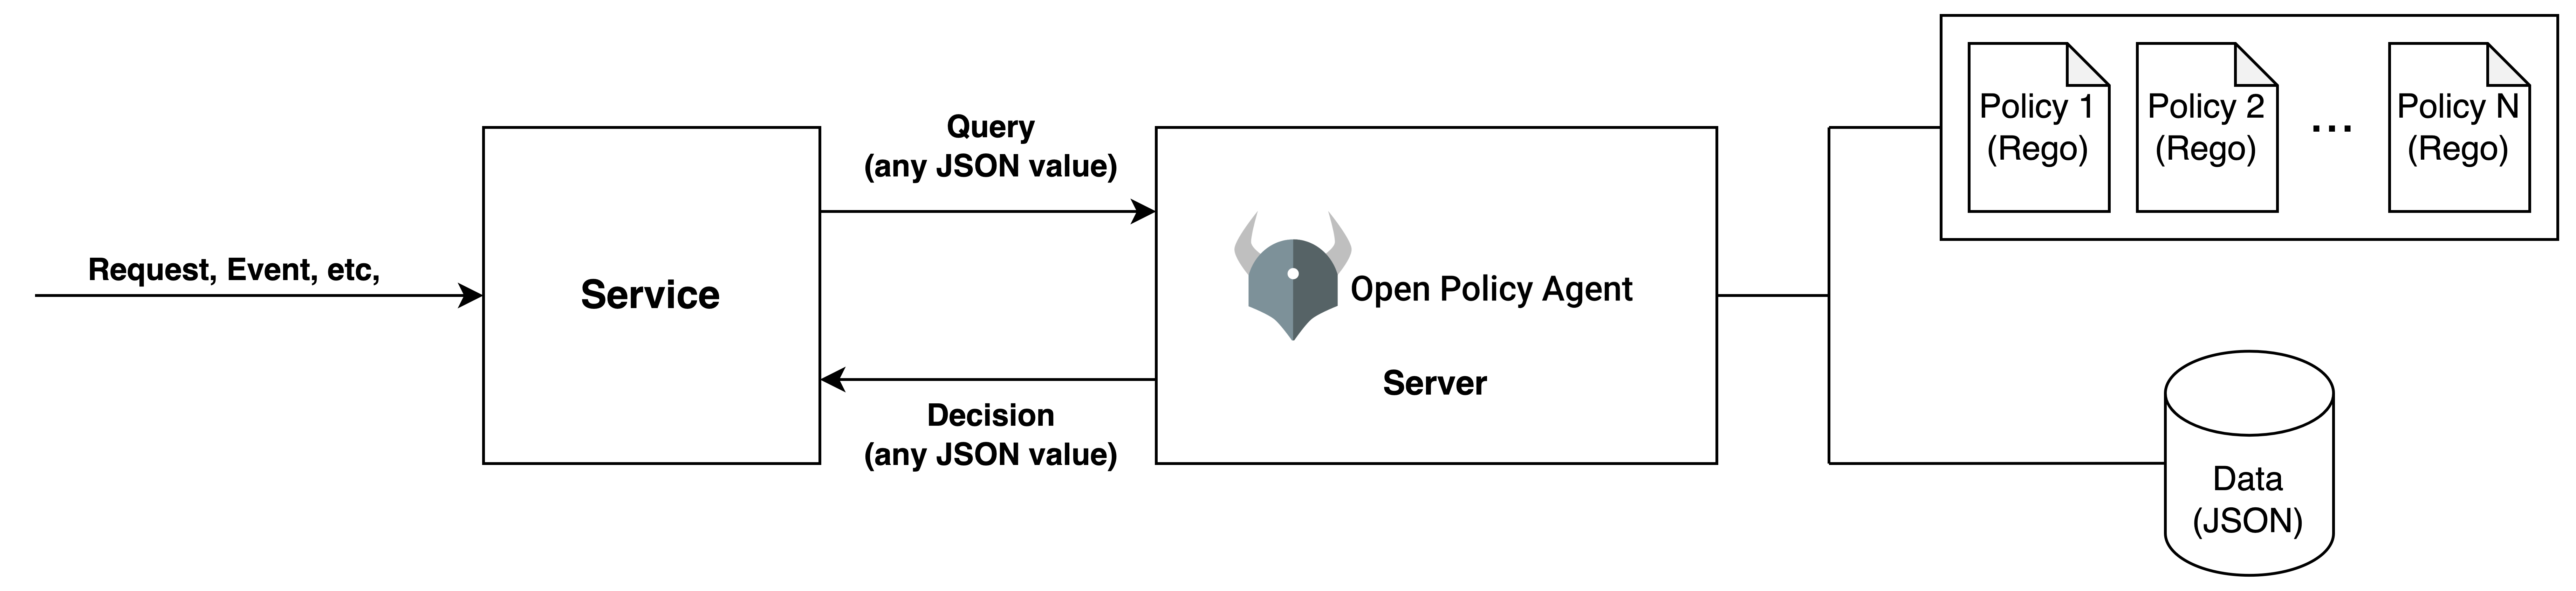
\includegraphics[width=1\linewidth]{images/OPA.png}
\caption{OPA architecture}
\label{fig:opa_architecture}
\end{figure}


OPA accepts arbitrary structured data as input.
and  Like query inputs, your policies can generate arbitrary structured data as output.

\subsection{OPA and external data}

types of external data strategies

http.send()
paramters 

\subsection{OPA integration with Kubernetes}

In Kubernetes admission control, policy enforcement is handled by the \textbf{Kubernetes API server} itself. OPA makes the policy decisions when queried by the admission controller, but the actual enforcement (namely allowing or denying requests) is executed by Kubernetes' built-in admission control mechanisms. This workflow is represented in figure \ref{fig:webhook_opa} where \textbf{AdmissionrReview request} and \textbf{AdmissionReview response} are respectively input and output of the whole OPA section. The API Server sends the entire Kubernetes object in the webhook request to OPA. %cite OPA kubernetes primer
The Kubernetes API server will use the received AdmissionReview response for its decision. \\
%\cite{opa_philosophy}

% https://www.openpolicyagent.org/docs/latest/kubernetes-tutorial/

\begin{figure}[htb]
\centering
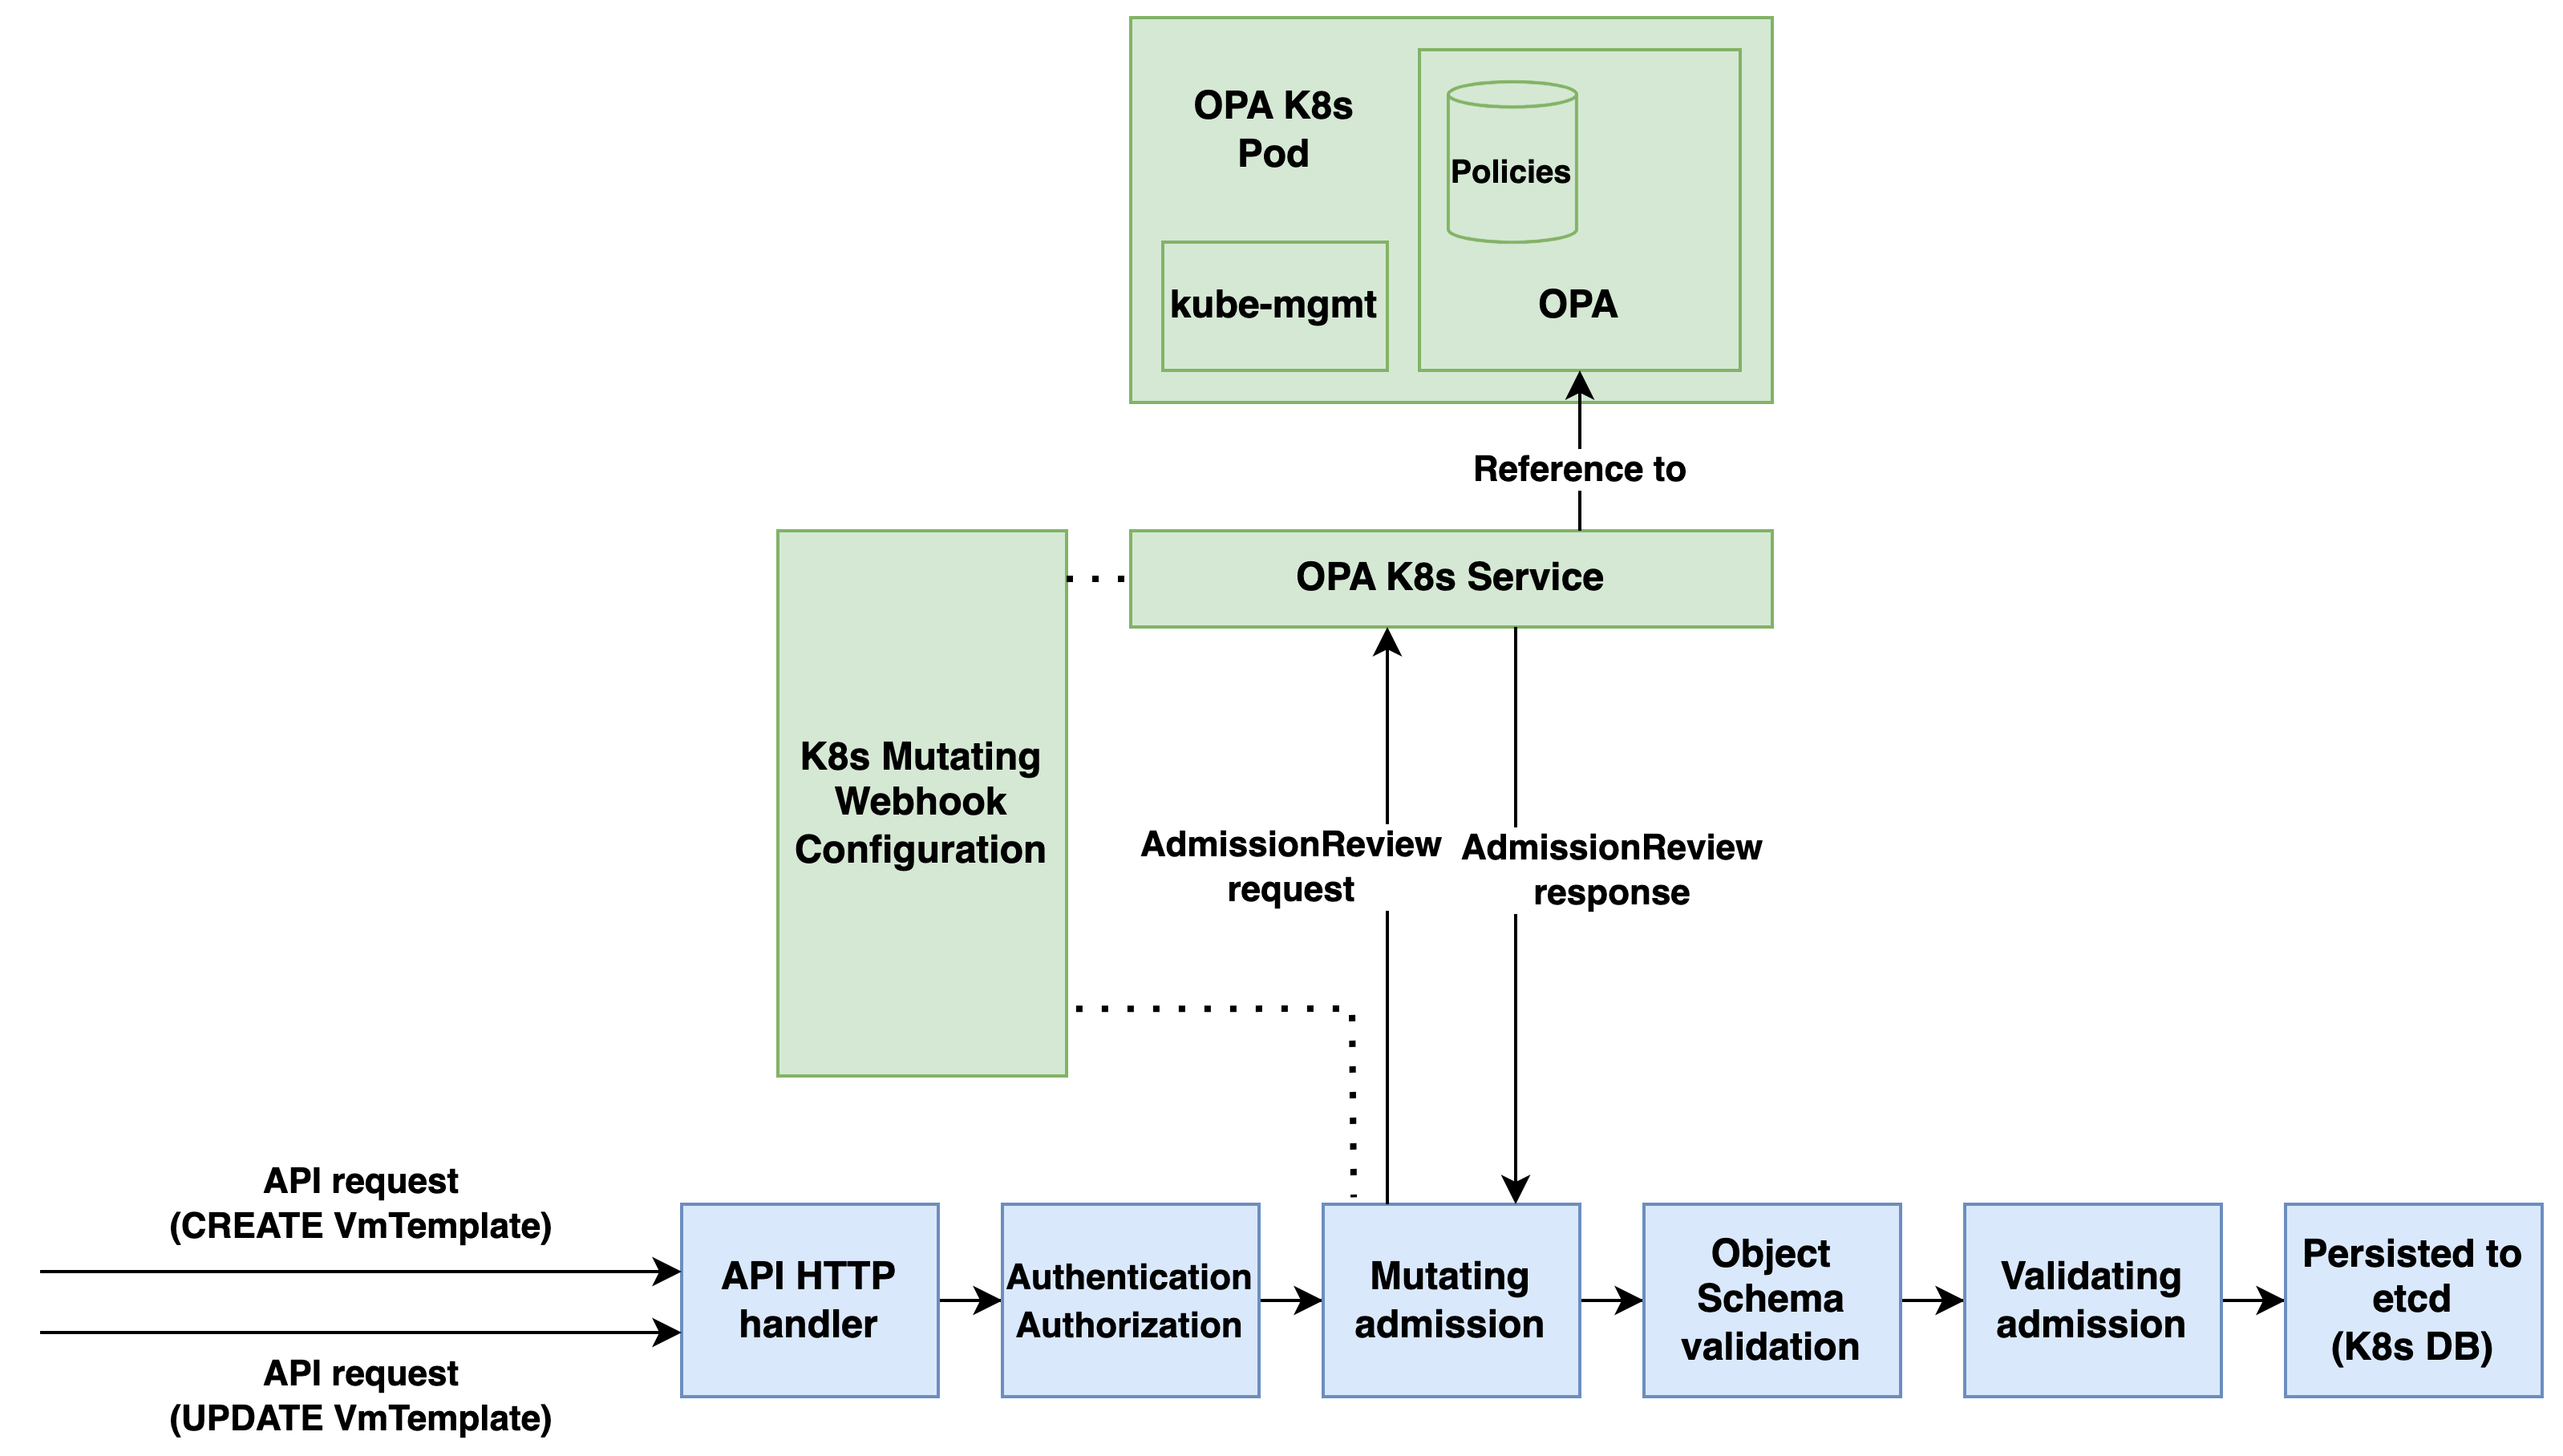
\includegraphics[width=1\linewidth]{images/webhook.png}
\caption{Kubernetes mutating webhook and OPA integration}
\label{fig:webhook_opa}
\end{figure}

In a Kubernetes deployment, an OPA Pod typically consists of the following containers:
\begin{itemize}[itemsep=0.2pt, topsep=1pt]
  \item[$\bullet$] OPA server container
  \item[$\bullet$] \textbf{kube-mgmt} container \\
\end{itemize} 

The kube-mgmt container functions as a \textbf{sidecar container} within a Kubernetes Pod. The sidecar container pattern is a common Kubernetes design paradigm in which auxiliary containers run alongside the main application container within the same Pod. These additional containers serve to enhance, extend, or support the primary application's functionality without modifying its core logic \cite{sidecar_containers}. 
The primary responsibility of kube-mgmt is to replicate Kubernetes resources into the OPA instance (OPA container). This operation is essential for OPA to access and evaluate policies based on real-time cluster state, enabling dynamic policy enforcement. By synchronizing these resources, kube-mgmt ensures that OPA has an up-to-date view of relevant Kubernetes objects.
This is especially useful to enforce policies that deals with naming conflicts, where OPA needs to check existing names in the cluster for the decision \cite{kube-mgmt}.
Additionally, it allows for loading policies directly from the Kubernetes cluster by retrieving them in the form of ConfigMaps. This feature is particularly useful when policies need to be dynamically updated based on the current state of the cluster \cite{kube-mgmt}. However, in the system described in this thesis, this latter feature is not employed in the current implementation as we are using policy bundles for policy distribution.

In the current system configuration, the kube-mgmt container is deployed to facilitate resource replication, ensuring that Kubernetes resources, namely VmTemplate resources, are synchronized with the OPA instance. However, at present, no policy requires interrogation of VmTemplate resources that are already present in the system.
Looking ahead, future policies could leverage VmTemplate resource information to enforce naming conflict resolution, quota management, or additional constraints.

\newpage

\subsection{OPA policies}
\label{sec:opa_policies}

%example of a policy:
%(https://www.openpolicyagent.org/docs/latest/kubernetes-primer/)





As OPA official documentation describes, when the Kubernetes AdmissionReview request from the webhook arrives, it is binded to the OPA input document and generates the default, ``root", decision: \textit{system.main}
%\cite

The root policy, in the case of Kubernetes admission control, is responsible for generating the AdmissionReview response in accordance with the Kubernetes API specifications. It is the duty of the policy developer to write Rego code that produces a well-formed AdmissionReview response, ensuring that the OPA server can then correctly communicate its decision to the Kubernetes admission controller.
%cite

It is deemed useful to show one of the simplest and common example of a OPA policy in the \textbf{Kubernetes admission control context}. That is: to ensure all images for Kubernetes Pods come from a trusted registry, namely \textit{unitn.it}. \\


It is important to note that, in this case, due to the simplicity of the policy, no additional contextual data in JSON format is required.


policy compilation
policy are compiled
compile time errors like merge errors if data is clashing for instance



\begin{comment}
    \lstset{
   language=Go,
   basicstyle=\ttfamily\small,
   breaklines=true,
   showstringspaces=false,
   commentstyle=\color{green!60!black},
   keywordstyle=\color{blue},
   stringstyle=\color{purple},
   numberstyle=\tiny,
   numbers=left,
   backgroundcolor=\color{gray!10},
   frame=single,
   captionpos=b
}
\end{comment}


\begin{lstlisting}[language=Rego, caption={Rego policy for Pods registry},
label=lst:rego_data_mapping]                              
deny contains msg if {                                                      
    input.request.kind.kind == "Pod"                                        
    image := input.request.object.spec.containers[_].image                  
    not startswith(image, "unitn.it/")                                     
    msg := sprintf("image '%v' comes from untrusted registry", [image])     
}
\end{lstlisting}

\begin{lstlisting}[language=Rego, caption={Rego ``root" policy (system.main)}]
package system

import data.kubernetes.admission

main := {
	"apiVersion": "admission.k8s.io/v1",
	"kind": "AdmissionReview",
	"response": response,
}

default uid := ""

uid := input.request.uid

response := {
	"allowed": false,
	"uid": uid,
	"status": {"message": reason},
} if {
	reason := concat(", ", admission.deny)
	reason != ""
}

else := {"allowed": true, "uid": uid}
\end{lstlisting}


\newpage
\lstset{style=jsonstyle}
\begin{lstlisting}[caption={AdmissionReview request}]
{
    "apiVersion": "admission.k8s.io/v1",
    "kind": "AdmissionReview",
    "request": {
        "kind": {
            "group": "",
            "kind": "Pod",
            "version": "v1"
        },
        "object": {
            "metadata": {
                "name": "myapp"
            },
            "spec": {
                "containers": [
                    {
                        "image": "bitnami/node:22",
                        "name": "nodejs"
                    }
                ]
            }
        }
    }
}
\end{lstlisting}

\lstset{style=jsonstyle}
\begin{lstlisting}[caption={AdmissionReview response}]
{
    "apiVersion": "admission.k8s.io/v1",
    "kind": "AdmissionReview",
    "response": {
        "allowed": false
        "status": {
            "message": "image 'bitnami/node:22' comes from untrusted registry"
        }
    }
}
\end{lstlisting}

Therefore, in this specific case, the creation of the Kubernetes Pod will be \textbf{denied}. OPA is responsible for \textbf{decision-making}, determining that the request do not complies with the defined policies, while the Kubernetes API server, using the AdmissionReview response generated by OPA, handles \textbf{policy enforcement}, effectively rejecting the CREATE request since it violates the specified rules.

\subsection{OPA Policy bundles}
\label{sec:opa_bundles}

An OPA policy bundle is a collection of policies and optional associated contextual data. More precisely, a bundle is a standardized way to package policies, facilitating version control and distribution \cite{opa_bundles}. As a matter of fact, a single policy bundle can be potentially used by multiple OPA instances.
A policy bundle mainly consists of:
\begin{itemize}[itemsep=0.2pt, topsep=1pt]
  \item[$\bullet$] \textbf{Rego policy files} defining the logic.
  \item[$\bullet$] \textbf{Data files} (in JSON or YAML format) containing contextual information required for policy evaluation (e.g., cloud region mappings).
\end{itemize} 

Policy bundles can be distributed through a variety of mechanisms such as remote HTTP servers (e.g., NGINX) and object storage services (e.g., Amazon S3, Google Cloud Storage, Azure Blob Storage) \cite{opa_bundles}.
One of the most convenient approaches is packaging them as \textbf{OCI (Open Container Initiative) images} \cite{oci} and this is the approach adopted in the system described in this thesis.

Once packaged as OCI images, policy bundles can be pulled by OPA servers from a container registry at predefined time intervals. This allows policy updates to be deployed in OPA \textbf{without requiring manual intervention} or \textbf{service restarts}, ensuring that enforcement mechanisms remain up to date with the latest compliance requirements identified and implemented by the organization. This is crucial for instance when dealing with \textbf{critical security policies} that need to be updated frequently, maybe in response to the discoveries of new CVEs. In the context of our system, such timely updates are not essential but the OPA is designed to be able to handle them if needed.
To ensure continuous policy enforcement while maintaining high operational efficiency, a CI/CD approach is adopted for policy management in the context of our system.
As a matter of fact, policies are maintained in a \textbf{version-controlled hosted repository} (i.e., on GitHub), where updates like tagging (``git tag'') trigger an automated pipeline (e.g., using GitHub Actions) responsible for building, packaging into a OCI image, and publishing the policy bundle to a container registry (e.g., Docker Hub).
One of the major advantages of this approach is the ability to dynamically update policies without requiring OPA pods to restart as there is an \textbf{hot-reload} of policies done at application level by OPA (``loaded on the fly'') \cite{opa_bundles}. This is particularly useful in production environments where service availability is critical and downtime must be minimized. 
The overall process of policy distribution is illustrated in figure \ref{fig:opa_bundles}.

\begin{figure}[H]
\centering
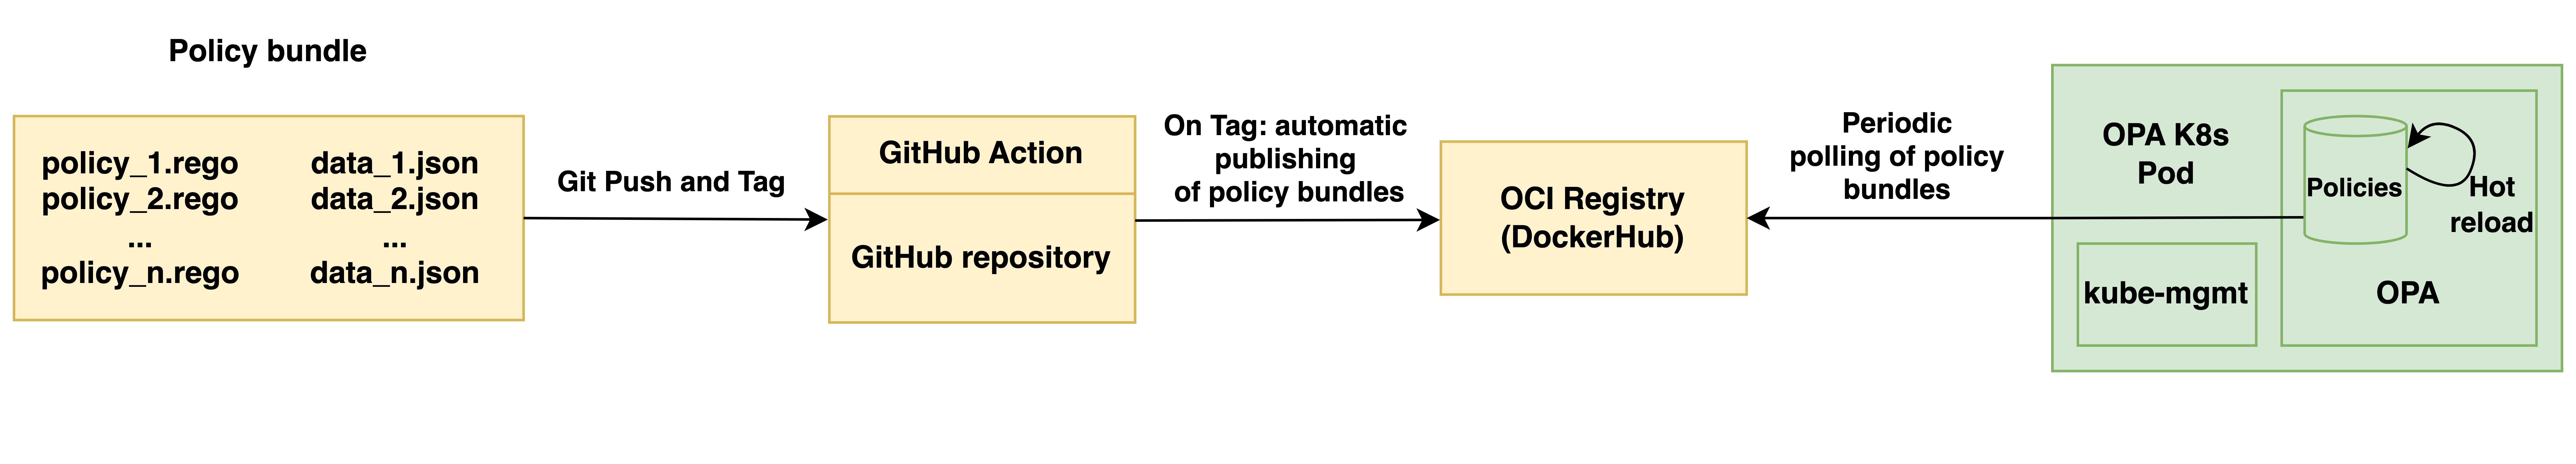
\includegraphics[width=1\linewidth]{images/opa_bundles.png}
\caption{OPA policy bundles}
\label{fig:opa_bundles}
\end{figure}

By leveraging OCI images for policy distribution and implementing a fully automated CI/CD pipeline, our system ensures that policy enforcement remains consistent, up to date, and highly available across all OPA instances. This approach aligns with modern DevOps practices, enabling organizations to maintain a high level of security and compliance without compromising operational efficiency.

\newpage

\subsection{OPA Gatekeeper}

OPA Gatekeeper is a Kubernetes-native policy engine that extends OPA with \textbf{Custom Resources (CRs)} and controllers to enforce policies across a Kubernetes cluster. It integrates natively with Kubernetes and provides a declarative approach to defining and enforcing policies using Kubernetes Custom Resources (CRs). This makes it an excellent choice for basic and standard policy enforcement scenarios, such as RBAC (Role-Based Access Control), security compliance, and resource constraints.
However, while OPA Gatekeeper is well-suited for simple use cases, it presents \textbf{limitations} when addressing complex policy requirements, particularly when policies involve \textbf{mutations} or require access to \textbf{external data sources}. These limitations make it unsuitable for the specific challenges tackled in this system. Therefore, after an initial investigation and Proof of Concept implementation, we decided to use the standard OPA server for policy enforcement mainly due to the flexibility it provides in handling diverse scenarios.

To illustrate the differences between a standard OPA policy and an OPA Gatekeeper policy, we present two examples:  
\begin{itemize}[itemsep=0.2pt, topsep=1pt]
  \item[$\bullet$] a simple Rego policy that enforces a basic constraint on Pod creation in a Kubernetes cluster.
  \item[$\bullet$] the corresponding policy implemented as an OPA Gatekeeper \textbf{ConstraintTemplate} and \textbf{Constraint} Kubernetes resources.
\end{itemize}

The first example demonstrates a standalone Rego policy, which can be evaluated directly by an OPA instance. While this approach is flexible and allows for fine-grained policy definition, it requires manual integration into the system, including policy distribution and enforcement setup.  

\lstset{style=python}
\begin{lstlisting}[language=rego, caption={Simple OPA Rego Policy}, label={lst:opa-rego}]
package kubernetes.admission

deny[msg] {
  input.request.kind.kind == "Pod"
  input.request.object.metadata.namespace == "restricted"
  msg := "Pods cannot be created in the 'restricted' namespace."
}
\end{lstlisting}

The second example, illustrated in listing \ref{lst:gatekeeper-template} utilizes OPA Gatekeeper, which extends Kubernetes with Kubernetes-native Custom Resource Definitions (CRDs), enabling declarative policy management. By using a ConstraintTemplate, policies can be enforced dynamically through Kubernetes, making them easier to distribute and manage.
In other words, with this kind of setting, OPA policy bundles are not employed in the same way as in the standard OPA server. Instead, policies are defined as Kubernetes resources, allowing for more straightforward policy enforcement and management within a Kubernetes environment.

\begin{lstlisting}[language=yaml, caption={OPA Gatekeeper ConstraintTemplate}, label={lst:gatekeeper-template}]
apiVersion: templates.gatekeeper.sh/v1
kind: ConstraintTemplate
metadata:
  name: podnamespaceconstraint
spec:
  crd:
    spec:
      names:
        kind: PodNamespaceConstraint
  targets:
    - target: admission.k8s.gatekeeper.sh
      rego: |
        package kubernetes.admission
        deny[msg] {
          input.review.object.metadata.namespace == "restricted"
          msg := "Pods cannot be created in the 'restricted' namespace."
        }
\end{lstlisting}

\begin{lstlisting}[language=yaml, caption={OPA Gatekeeper Constraint}, label={lst:gatekeeper-constraint}, float=htpb]
apiVersion: constraints.gatekeeper.sh/v1beta1
kind: PodNamespaceConstraint
metadata:
  name: restrict-namespace
spec:
  match:
    kinds:
      - apiGroups: [""]
        kinds: ["Pod"]
  parameters: {}
\end{lstlisting}

In the example, the policy is defined as a ConstraintTemplate, which is then instantiated as a Constraint Custom Resource of kind defined in the ConstraintTemplate. The ConstraintTemplate specifies the Rego policy logic, while the Constraint defines the target resources and parameters for policy enforcement. Therefore a ConstraintTemplate can be used by multiple Constraints, allowing for policy reuse.

OPA Gatekeeper also provides additional Kubernetes Custom Resources called \textit{mutators} (Assign, AssignMetadata, AssignImage, ModifySet) that allow modifying resource fields without writing Rego code. These mutators are useful for simple transformations, such as setting default labels or annotations. However simultaneous mutation of multiple fields leveraging external data is not supported \cite{opa_gatekeeper_external_data}. This limitation, in the context of our system, determined the choice of the standard OPA server for policy enforcement.

It must be noted that OPA Gatekeeper limitations could be potentially addressed in future releases, making it a more viable option for complex policy enforcement scenarios. However, for the current system requirements, the standard OPA server was deemed more suitable due to its flexibility.

\subsection{Latency policy}

A representative example of a policy aligned with Service Level Objectives (SLOs) or Service Level Agreements (SLAs) is the latency policy described in this section.
Given an \textbf{origin region} and a \textbf{maximum latency threshold} (expressed in milliseconds), the objective is to determine a \textbf{set of eligible regions} where the inter-regional latency between the origin and each region in the set is equal to or below the specified threshold.
Enforcing such constraints helps mitigate the so-called ``\textbf{black hole phenomenon}" in the GreenOps use case, where all virtual machines (VMs) would otherwise be scheduled in a region with generally low carbon intensity, without considering additional constraints or performance requirements. By incorporating similar performance-aware policies, organizations can achieve a balance between environmental impact, performance, and service reliability.
The proposed flexible system enables organizations to fine-tune these factors according to their specific requirements or those of their users. 
This policy demonstrates the flexibility of OPA in handling diverse compliance scenarios. It is the responsibility of the policy developer to design an appropriate strategy for encoding relevant information into \textbf{well-structured JSON data models}, e.g., a latency matrix. Proper structuring ensures efficient policy evaluation, maintainability and extendability.

Figure \ref{fig:latency_matrix} illustrates an small example (4 regions subset) of a latency matrix, where each cell represents the latency between two regions. The matrix can be encoded in JSON format as illustrated in listing \ref{lst:latency_matrix_example}, allowing for easy integration with OPA policies. The ``Latency policy'' then uses this matrix to determine eligible regions based on the origin region and maximum latency threshold.

\begin{figure}[H]
  \centering
  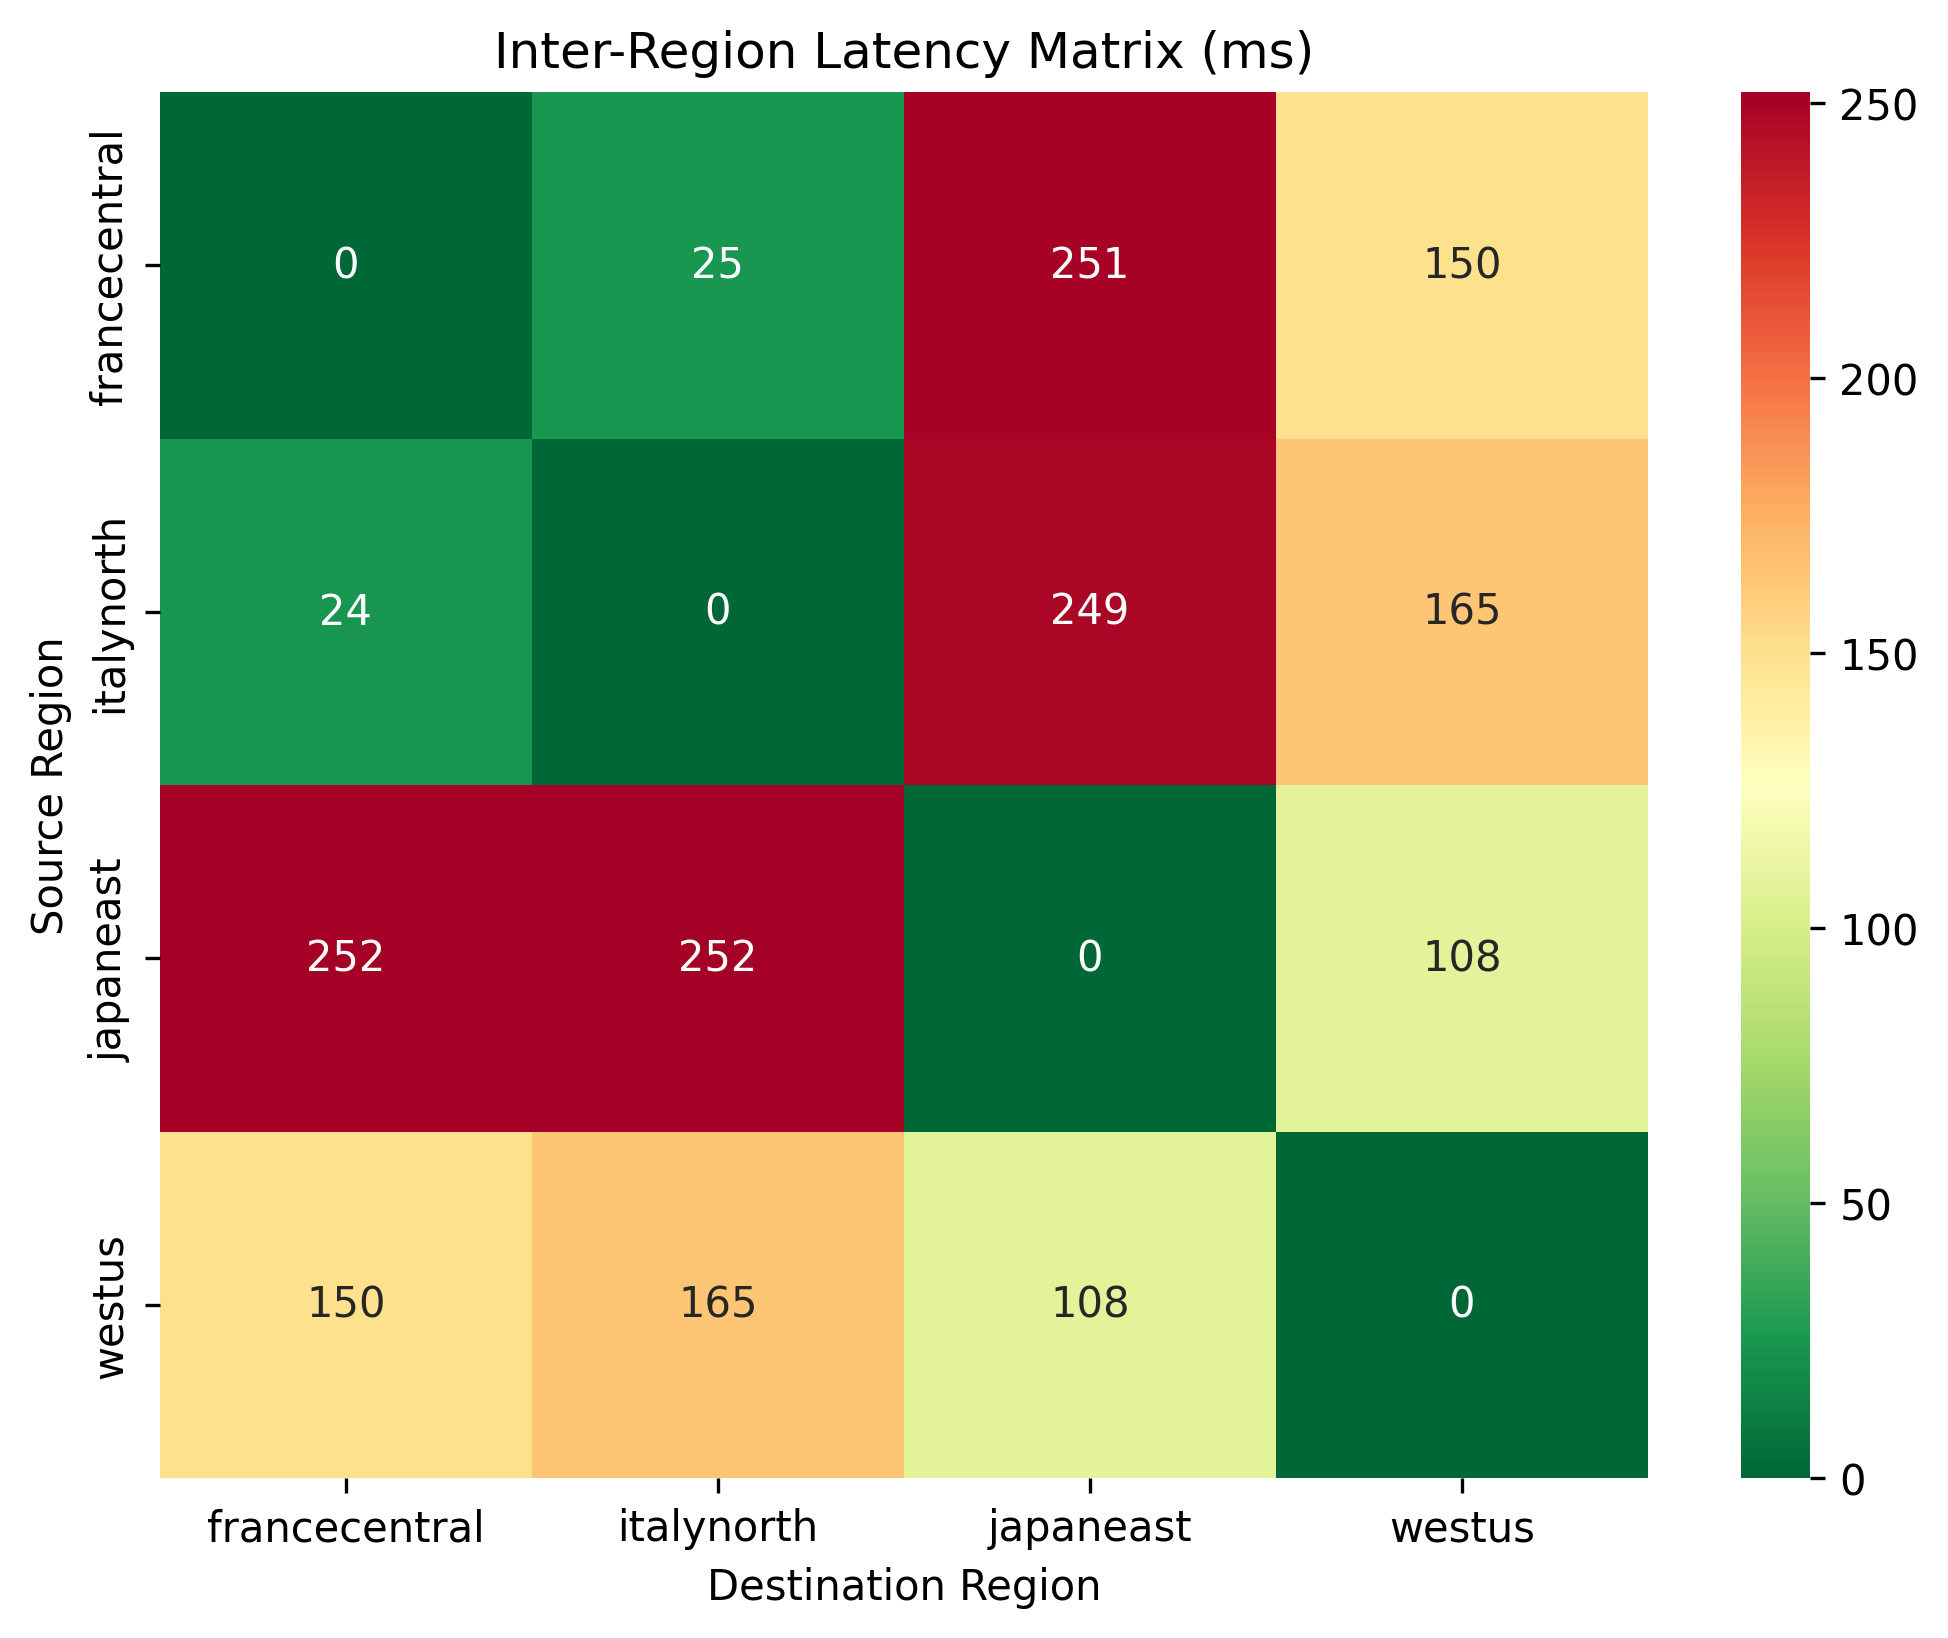
\includegraphics[width=0.75\linewidth]{images/latency_heatmap.png}
  \caption{Latency matrix example (Azure regions subset)}
  \label{fig:latency_matrix}
\end{figure}


\lstset{style=jsonstyle}
\begin{lstlisting}[caption={Latancy matrix example encoded in JSON format}, label={lst:latency_matrix_example}]
  {
    "italynorth": {
        "italynorth": 0,
        "japaneast": 249,
        "francecentral": 24,
        "westus": 165
    },
    "japaneast": {
        "italynorth": 252,
        "japaneast": 0,
        "francecentral": 252,
        "westus": 108
    },
    "francecentral": {
        "italynorth": 25,
        "japaneast": 251,
        "francecentral": 0,
        "westus": 150
    },
    "westus": {
        "italynorth": 165,
        "japaneast": 108,
        "francecentral": 150,
        "westus": 0
    }
}

\end{lstlisting}


data

Azure provides monthly Percentile P50 round trip times between Azure regions:
(https://learn.microsoft.com/en-us/azure/networking/azure-network-latency?tabs=Americas%2CWestUS)
https://learn.microsoft.com/en-us/azure/networking/media/azure-network-latency/azure-network-latency-thumb.png#lightbox 

Azure network latencies docs:
https://raw.githubusercontent.com/MicrosoftDocs/azure-docs/refs/heads/main/articles/networking/azure-network-latency.md

Merged Azure network latencies:
https://docs.google.com/spreadsheets/d/1kxtPw9ZSnAv1vQ6IDwzw-mXdHoKUFb8AjlsjACnvDqE/edit?usp=sharing 


AWS:
https://www.cloudping.co/grid (not official, not using VMs but Lambda functions)
how it is calculated

google
syntetic data
no offical data



\subsection{GDPR policy}

Another policy configured in the system is the ``GDPR Policy'', which ensures that virtual machines (VMs) are deployed in cloud regions that reside in countries of the European Union. 
The policy is based on the principle of \textbf{set intersection}. One set consists of the eligible regions determined by other constraints, such as latency requirements. The other set includes cloud provider regions that are physically located within European Union (EU) countries.
The intersection of these two sets defines the final list of allowed deployment regions, restricting workloads to EU-based data centers.
Since each cloud provider has its own regional distribution, the list of EU-compliant regions is provider-specific and is encoded as contextual data in JSON format. This allows for flexibility and easy updates when cloud providers introduce new regions.

It must be noted that this policy is \textbf{not intended to be a comprehensive GDPR compliance solution}, but rather a basic example of how OPA can enforce \textbf{data residency requirements in a multi-cloud environment}. Organizations with more stringent GDPR compliance needs should consider additional measures.

\subsection{Scheduling outcome policy}

main policy

Mutation policy
dedicated to 



JSON Patch is a format for describing changes to a JSON document which avoid the need to send the entire document when only a part of it has changed. Effectively, only deltas are sent back to the requester which are themselves JSON documents.
The format is defined in RFC 6902 from the IETF \cite{json_patch}.

As an example, a single patch operation 


OPA, assuming the role of a webhook server, has the duty of ..





\subsection{OPA Data mapping}

OPA is flexible enough to handle data mapping between different data models, enabling seamless integration with external systems. In our GreenOps system, data mapping is essential for translating between ElectricityMaps regions and cloud provider regions. 


At some point in the system this mapping needs to be done.
this mappings are needed since the scheudler knows only about ElectricityMaps regions, and do not possess the knowledge of cloud provider regions. Therefore, a mapping is needed to translate the ElectricityMaps regions to cloud provider regions and vice versa.

inside the policy is a good place to do this mapping


first filter is the selection of the provider
this determine the whole set of regions belonging to that provider

eligible regions: this filter can be only done with cloud provider specific latencies

\begin{figure}[H]
  \centering
  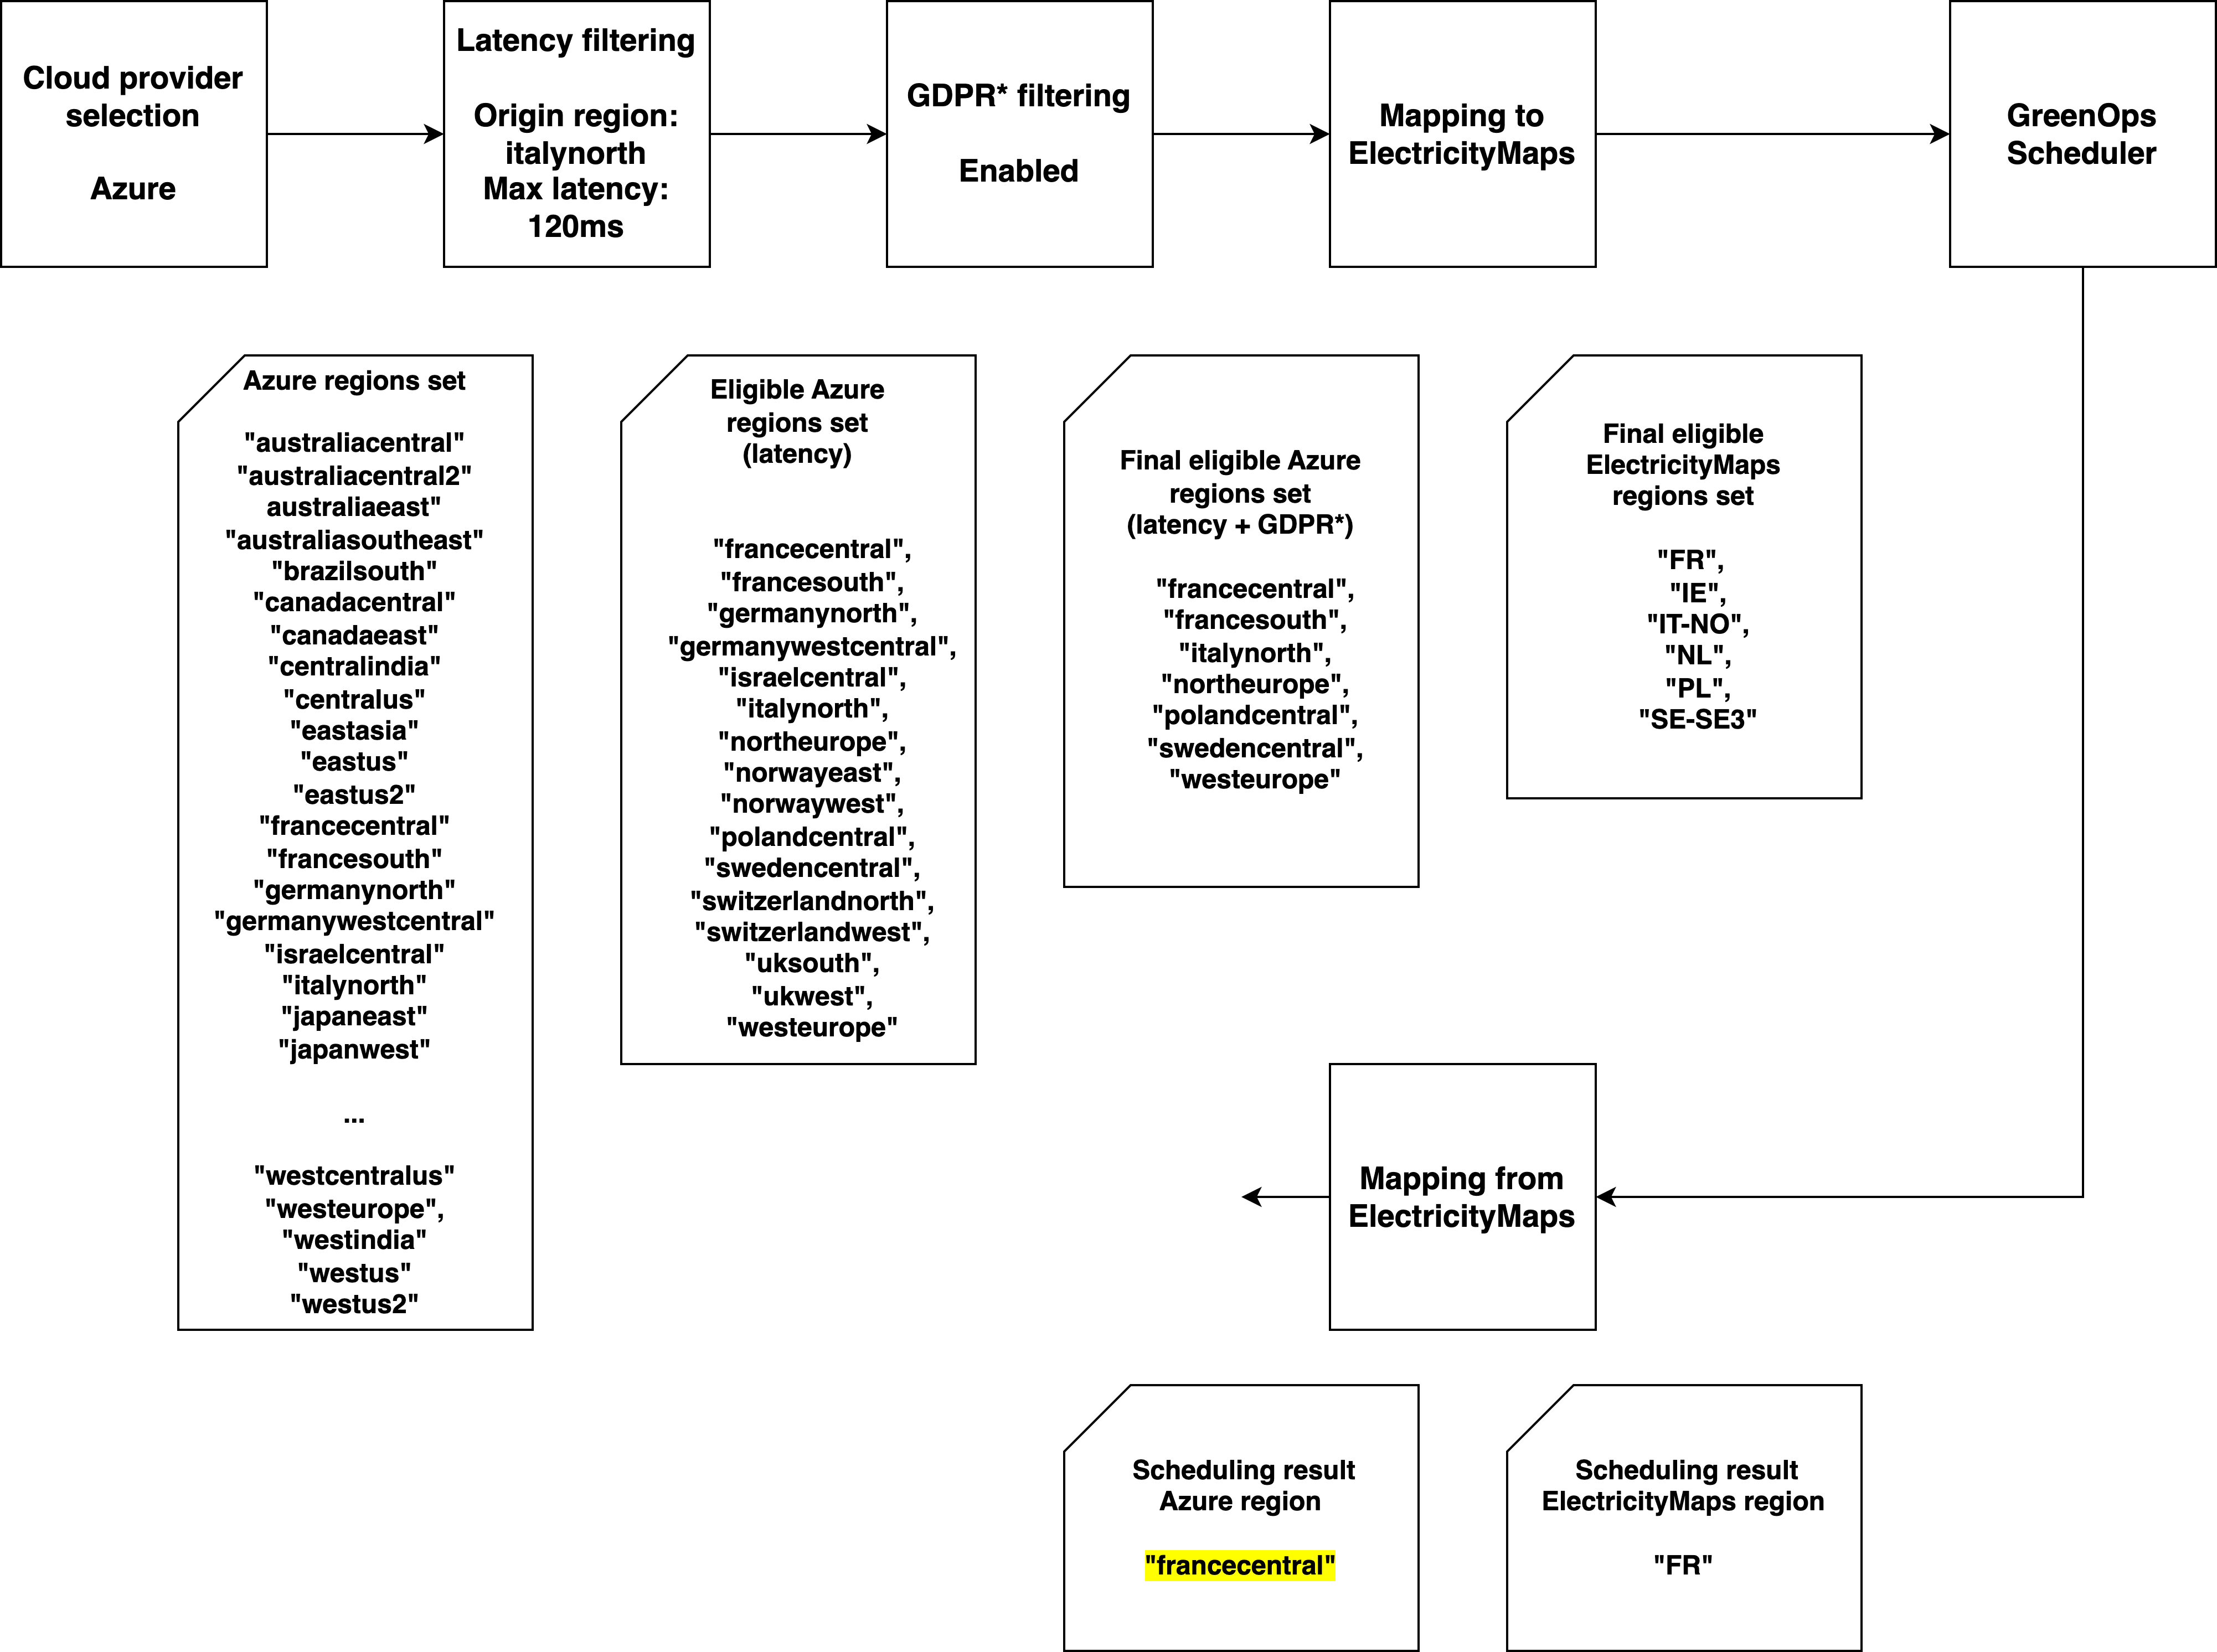
\includegraphics[width=1\linewidth]{images/data_mapping.png}
  \caption{OPA Data mapping}
  \label{fig:data_mapping}
\end{figure}


\begin{lstlisting}[language=Rego, caption=Rego data mapping, label=lst:rego_data_mapping]
# Utility functions to map between cloud provider regions 
# and ElectricityMaps regions

map_to_electricitymaps(eligible_regions, provider) = em_regions if {
    em_regions := {
        region.ElectricityMapsName |                             
        some eligible_region;                       
        some region;                                
        eligible_region = eligible_regions[_];      
        region = data[provider].cloud_regions[_];   
        region.Name == eligible_region             
        region.ElectricityMapsName != ""            
        region.ElectricityMapsName != "Unknown"
    }
}

map_from_electricitymaps(em_region, provider) = cloud_region if {
    some region;                              
    region = data[provider].cloud_regions[_];   
    region.ElectricityMapsName == em_region;    
    cloud_region := region.Name 
}

\end{lstlisting}

\subsection{OPA end-to-end workflow}

 (K8s mutating webhook)

OPA flow:

- admission review (contains max\_latency, origin\_region)

- policy contains cloud provider (or chose for the user)

- policy calculate subset of eligible regions

- policy will ask scheduling information to the scheduler (using http.send()










relationship with k8s mutating webhook

rego policies


scheduler has notions of 
electricity maps regions only

OPA is used also as a data mapping layer
both at request time
and at response time


\begin{figure}[htb]
\centering
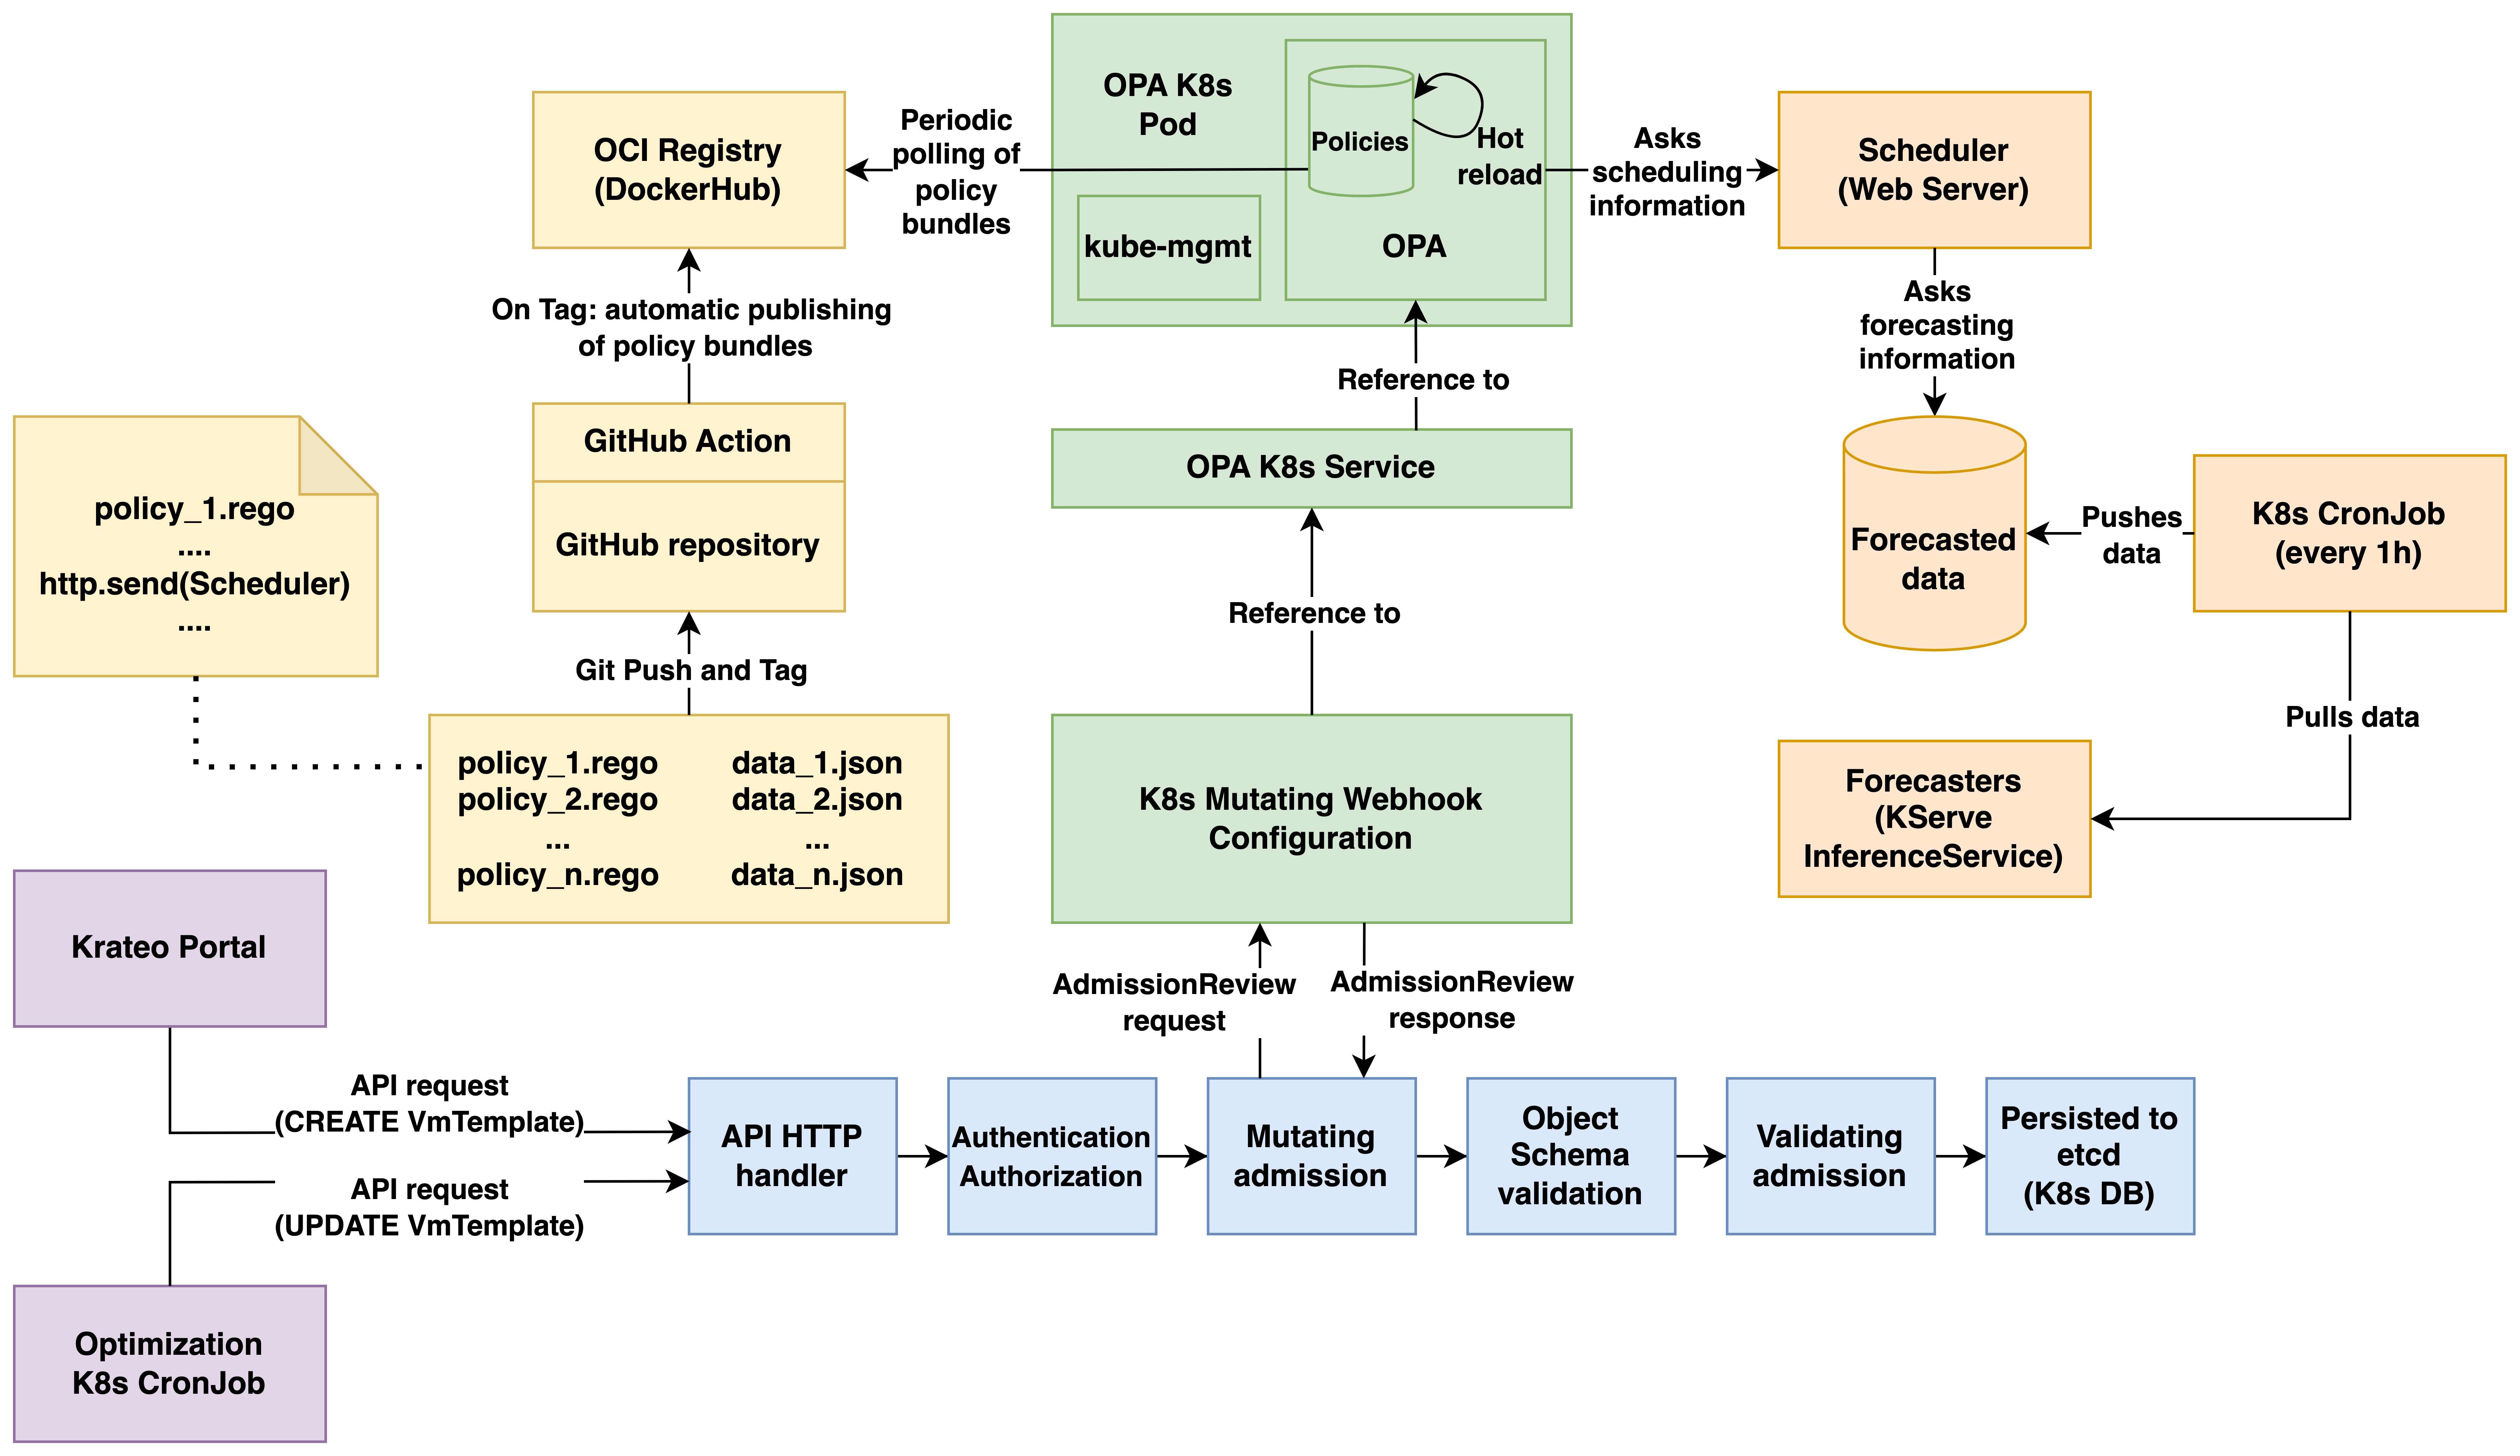
\includegraphics[width=1\linewidth]{images/mutating_webhook+OPA_integration.png}
\caption{Kubernetes mutating webhook + OPA integration}
\label{fig:webhook+opa}
\end{figure}

Figure \ref{fig:webhook+opa} represents the configuration of the Kubernetes Mutating Webhook with the intergeation of Open Policy Agent.
In particular, 




Day 2 operations
what are day 2 operations: in this case (VMs) resize a VM (scale up or down) based on the load
The mutating webhook configuration is set on the CREATE and UPDATE operations

UPDATE operation trigger
K8s Cronjob that attach a label to the custom resoruce 

\subsection{OPA advanced features}

It is deemed useful to mention some of the advanced features of OPA that were not employed in the system described in this thesis but could be potentially useful in future developments or in other contexts where OPA is used.

- bundle signing
- delta bundles

\newpage

\section{MLOps infrastructure}

A MLOps infrastrcutrue is not necessarily needed for multi-cloud resource management but since it is believed that AI models will be used in the future more and more to get scheduling and management decisions
as testified by recents works described in chapter XXX.
It is therefore deemed important to describe a MLOps infrastructure in a Kubernetes environment leveraged by the system described in this thesis.

\subsection{MLOps purpose}

MLOps implements DevOps principles, tools and practices into Machine Learning workflows 

purpose: industrialize ML models lifecycle
faster model development
faster model selection and deployment to production

\begin{itemize}[itemsep=0.2pt, topsep=1pt]
  \item[$\bullet$] model tracking (experiments, runs)
  \item[$\bullet$] model selection (model registry)
  \item[$\bullet$] model storage (in buckets)
  \item[$\bullet$] model deployment (inference)
\end{itemize}


allows all the team member to have visibility on the status of the ML models

Instead of having the so-called ``AI Inference Mock Server", treated as a black box returning a scheul;ding time and schedulingLocation

\begin{figure}[htb]
\centering
\includegraphics[width=1\linewidth]{images/mlops_workflow.png}
\caption{MLOps Architecture}
\label{fig:mlops}
\end{figure}


MLFlow framework
KServe framework


\subsection{MLflow}



MLflow Tracking Server


mlflow is compatible with many ML frameworks like sklearn, pythorch


what is a model tracking server
what is a model registry



Mlflow API calls
autolog function
infer signature 
important since store 

the end result is a self contained fodler with everythiong needed to deploy the model
it allows reproducibility 

The training script will also serialise our trained model, leveraging the MLflow Model format.


model/
├── MLmodel
├── model.pkl
├── conda.yaml
└── requirements.tx


additional challenge: CrateDB is not supported natively by mlflow framework
a CrateDB adapter / wrapper is devoloped and mantianed by cratedb community
CrateDB as metadata stoere


SeaweedFS as artifact store
MINio could be an alternative altough it has a restrictive license \cite{minio_license}.



MODEL signature




\subsubsection{Alternative configuration 1}

an alternative solution

watchdog
watchdog (pyhton package)

sidecar container

artifact store not needed

\subsubsection{Alternative configuration 2}

Another possible configuration could be the adoption of just CrateDB as both Metadata Store and Artifact Store.

This would be possible if
CrateDB supports blob storage but not object storage

This solution cannot be implemented yet due to 


\subsection{KServe}


KServe Inference Service

what is
inference server / model server


used to deploy the forecaster (ML model)


uses Istio and Knative under the hood
features: scaling to zero, etc


InferenceService with TorchServe runtime which is the default installed serving runtime for PyTorch models.

Kserve project proposes a standard protocol for inference servers.
The version 2 of the KServe Inference Protocol is the Open Inference Protocol.



\subsubsection{Open Inference Protocol}


\begin{table}[h!]
\centering
\begin{tabular}{|l|l|l|}
\hline
\textbf{API}    & \textbf{Verb} & \textbf{Path}                                                                                         \\ \hline
Inference       & POST          & v2/models/{[}/versions/\textless{}model\_version\textgreater{}{]}/infer                               \\ \hline
Model Ready     & GET           & v2/models/\textless{}model\_name\textgreater{}{[}/versions/{]}/ready                                  \\ \hline
Model Metadata  & GET           & v2/models/\textless{}model\_name\textgreater{}{[}/versions/\textless{}model\_version\textgreater{}{]} \\ \hline
Server Ready    & GET           & v2/health/ready                                                                                       \\ \hline
Server Live     & GET           & v2/health/live                                                                                        \\ \hline
Server Metadata & GET           & v2                                                                                                    \\ \hline
\end{tabular}
\end{table}





adopted by NVIDIA



multi model deployment



our strategy:
1 model per region
1 generic model? as fallback if specific model is not available?




Kserve "stack"

Kserve

in kserve 0.14.1
clusterservingruntimes
supported are 10
among which 
torchserve

clusterservingruntimes -> kserve-mlserver (supported models: sklearn, xgboost, lightgbm, mlflow)

mlserver

[chart to illustrate this]







serving runtimes

Seldon MLserver


accorgimenti: \\
model wrapping

\section{Measurements}


% https://dynamorio.org/google_workload_traces.html


\subsection{System / performance metrics}


how to measuere cloud resource systems


especially useful for ``day 2 operations''
scaling down a VM


Metrics collected could be:
CPU usage
memory usage.
These metrics are especially useful for the 2nd use case for instance: scaling down a VM.


Prometheus exporters (https://prometheus.io/docs/instrumenting/exporters/) + Prometheus scrapers for data collection.
Generic Prometheus exporters and scrapers already used for Krateo Composable FinOps leveraging specific K8s Custom Resources. These exporters are generic and can scrape arbitrary metrics configured in specific CRs (for instance, collecting VMs CPU consumption though Azure APIs).
From the Krateo Composable FinOps document: 
- “we transform all optimizations into a set of Kubernetes Custom Resources (CRs) to act upon newly found cost-related deficiencies. This allows us to use Kubernetes operators (explicitly coded to interact with cloud services) to monitor these metrics and act automatically to apply changes to remote resources.”

- “forward the optimization to the Krateo operator that manages the services that need to be optimized, for example, the Azure Operator to modify the size of a Virtual Machine;”

- “the optimization is automatically encoded in a CR for the finops-operator-vm-manager, which then analyzes it and decides how to manage the Virtual Machine. For example, it could scale up or down the virtual machine, stop it for the night, etc.”

From my current understanding, only Azure is available for now on the finops-operator-vm-manager. 
This operator is only able to: start; stop; deallocate; scale-up; scale-down.
So finops-operator-vm-manager operates on already provisioned virtual machines and it applies optimizations.

---



Cloud providers API (“hypervisor” / host level) to get CPU usage, memory usage
Azure monitoring REST API: https://learn.microsoft.com/en-us/azure/azure-monitor/essentials/rest-api-walkthrough?tabs=rest%2Cportal
https://learn.microsoft.com/en-us/rest/api/monitor/metrics/list?view=rest-monitor-2023-10-01&tabs=HTTP
https://learn.microsoft.com/en-us/azure/virtual-machines/monitor-vm 


Cloud providers agents
Azure Monitor Agent (https://learn.microsoft.com/en-us/azure/azure-monitor/agents/azure-monitor-agent-overview)
Google Ops Agent: “the primary agent for collecting telemetry from your Compute Engine instances” (https://cloud.google.com/monitoring/agent/ops-agent)


Standard agents/deamons manually installed the VMs (e.g. Prometheus node exporter, 
many metrics restricted by public cloud providers
not straightforward to automate the deployment


---

Challenges
Public Cloud Providers do not provide data about carbon intensity of a VM instance
Public Cloud Providers do not provide data about power consumption of a VM instance

Power consumption metrics
scaphandre: NOT supported by public cloud providers. “Public cloud providers do not expose the underlying RAPL sensors that scaphandre and other measurement tools rely on to track consumption”. (https://github.com/hubblo-org/scaphandre/issues/142)
https://hubblo-org.github.io/scaphandre-documentation/index.html

kepler: really interesting and quite mature project but works only with K8s resources inside the cluster (Nodes, Pods). Therefore not good for our use first case.
https://sustainable-computing.io/design/architecture/


manually estimate power consumption based on CPU utilization, memory usage. Could be a very difficult task. 
there is the TEADS metodology like 



---


Carbon metrics:
there is no adopted standard, there is not something similar to FOCUS yet;
there is a proposal for a specification (work in progress, not supported yet by Public Cloud Providers): 
https://github.com/Green-Software-Foundation/real-time-cloud 
https://github.com/Green-Software-Foundation/real-time-cloud/blob/main/Cloud_Region_Metadata_specification.md 


Public Cloud Providers monthly reports (probably not useful in this case)
Export Azure carbon optimization emissions data (Preview) (probably not fine-grained as we want)

Cloud Carbon Footprint
Uses cloud provider billing (AWS Cost and Usage Reports with Amazon Athena, GCP Billing Export Table using BigQuery, Azure Consumption 
Management API). Using these services costs.
Electricity Maps API integration is supported (for live grid carbon intensity)

 
aether calculation engine (https://aether.green/docs/methodologies/) 
only AWS and GCP supported, Azure not yet
uses AWS CloudWatch and Google monitoring
very small project
no live Grid Carbon Intensity Coefficient, they extrapolate data from “governative” data reports
https://aether.green/docs/methodologies/#grid-carbon-intensity-coefficient


carbond agent) (https://gitlab.com/sustainable-computing-systems/carbond)
installed on the machine


Example of a manual approach (not scalable due to tech specs research): https://devblogs.microsoft.com/sustainable-software/how-can-i-calculate-co2eq-emissions-for-my-azure-vm/ 

The critical point here is to get/calculate the energy consumed by a cloud instance, since there are a huge number of technical configurations to find, retrieve and use for calculations.



\subsection{Impact framework}

Impact framework (by green software foundation)

\section{End-to-End workflow}
\label{sec:e2eflow}

[TO BE CHANGED]
A user request for a workload arrives in Kubernetes / Krateo. 
The request shape is VM1 = (MinCPU=4vCPU, MinRAM=4GiB, D=12h)
As we can see the request is generic: it does not contain a specific cloud provider or a specific cloud region.
A K8s Custom Resource (CR) representing the workload is created.
mutating webhook intercepts the CREATE API request.
K8s mutating webhook retrieve and evaluate policies and in particular, the AI model inference is called and should return a decision with the region and scheduling time (time-shifting and geographical shifting).
OPA will use this decision to mutate the VM specification, adding the provider, the schedulingRegion and schedulingTime fields.
Krateo core provider / cdc


\begin{sidewaysfigure}
  \centering
  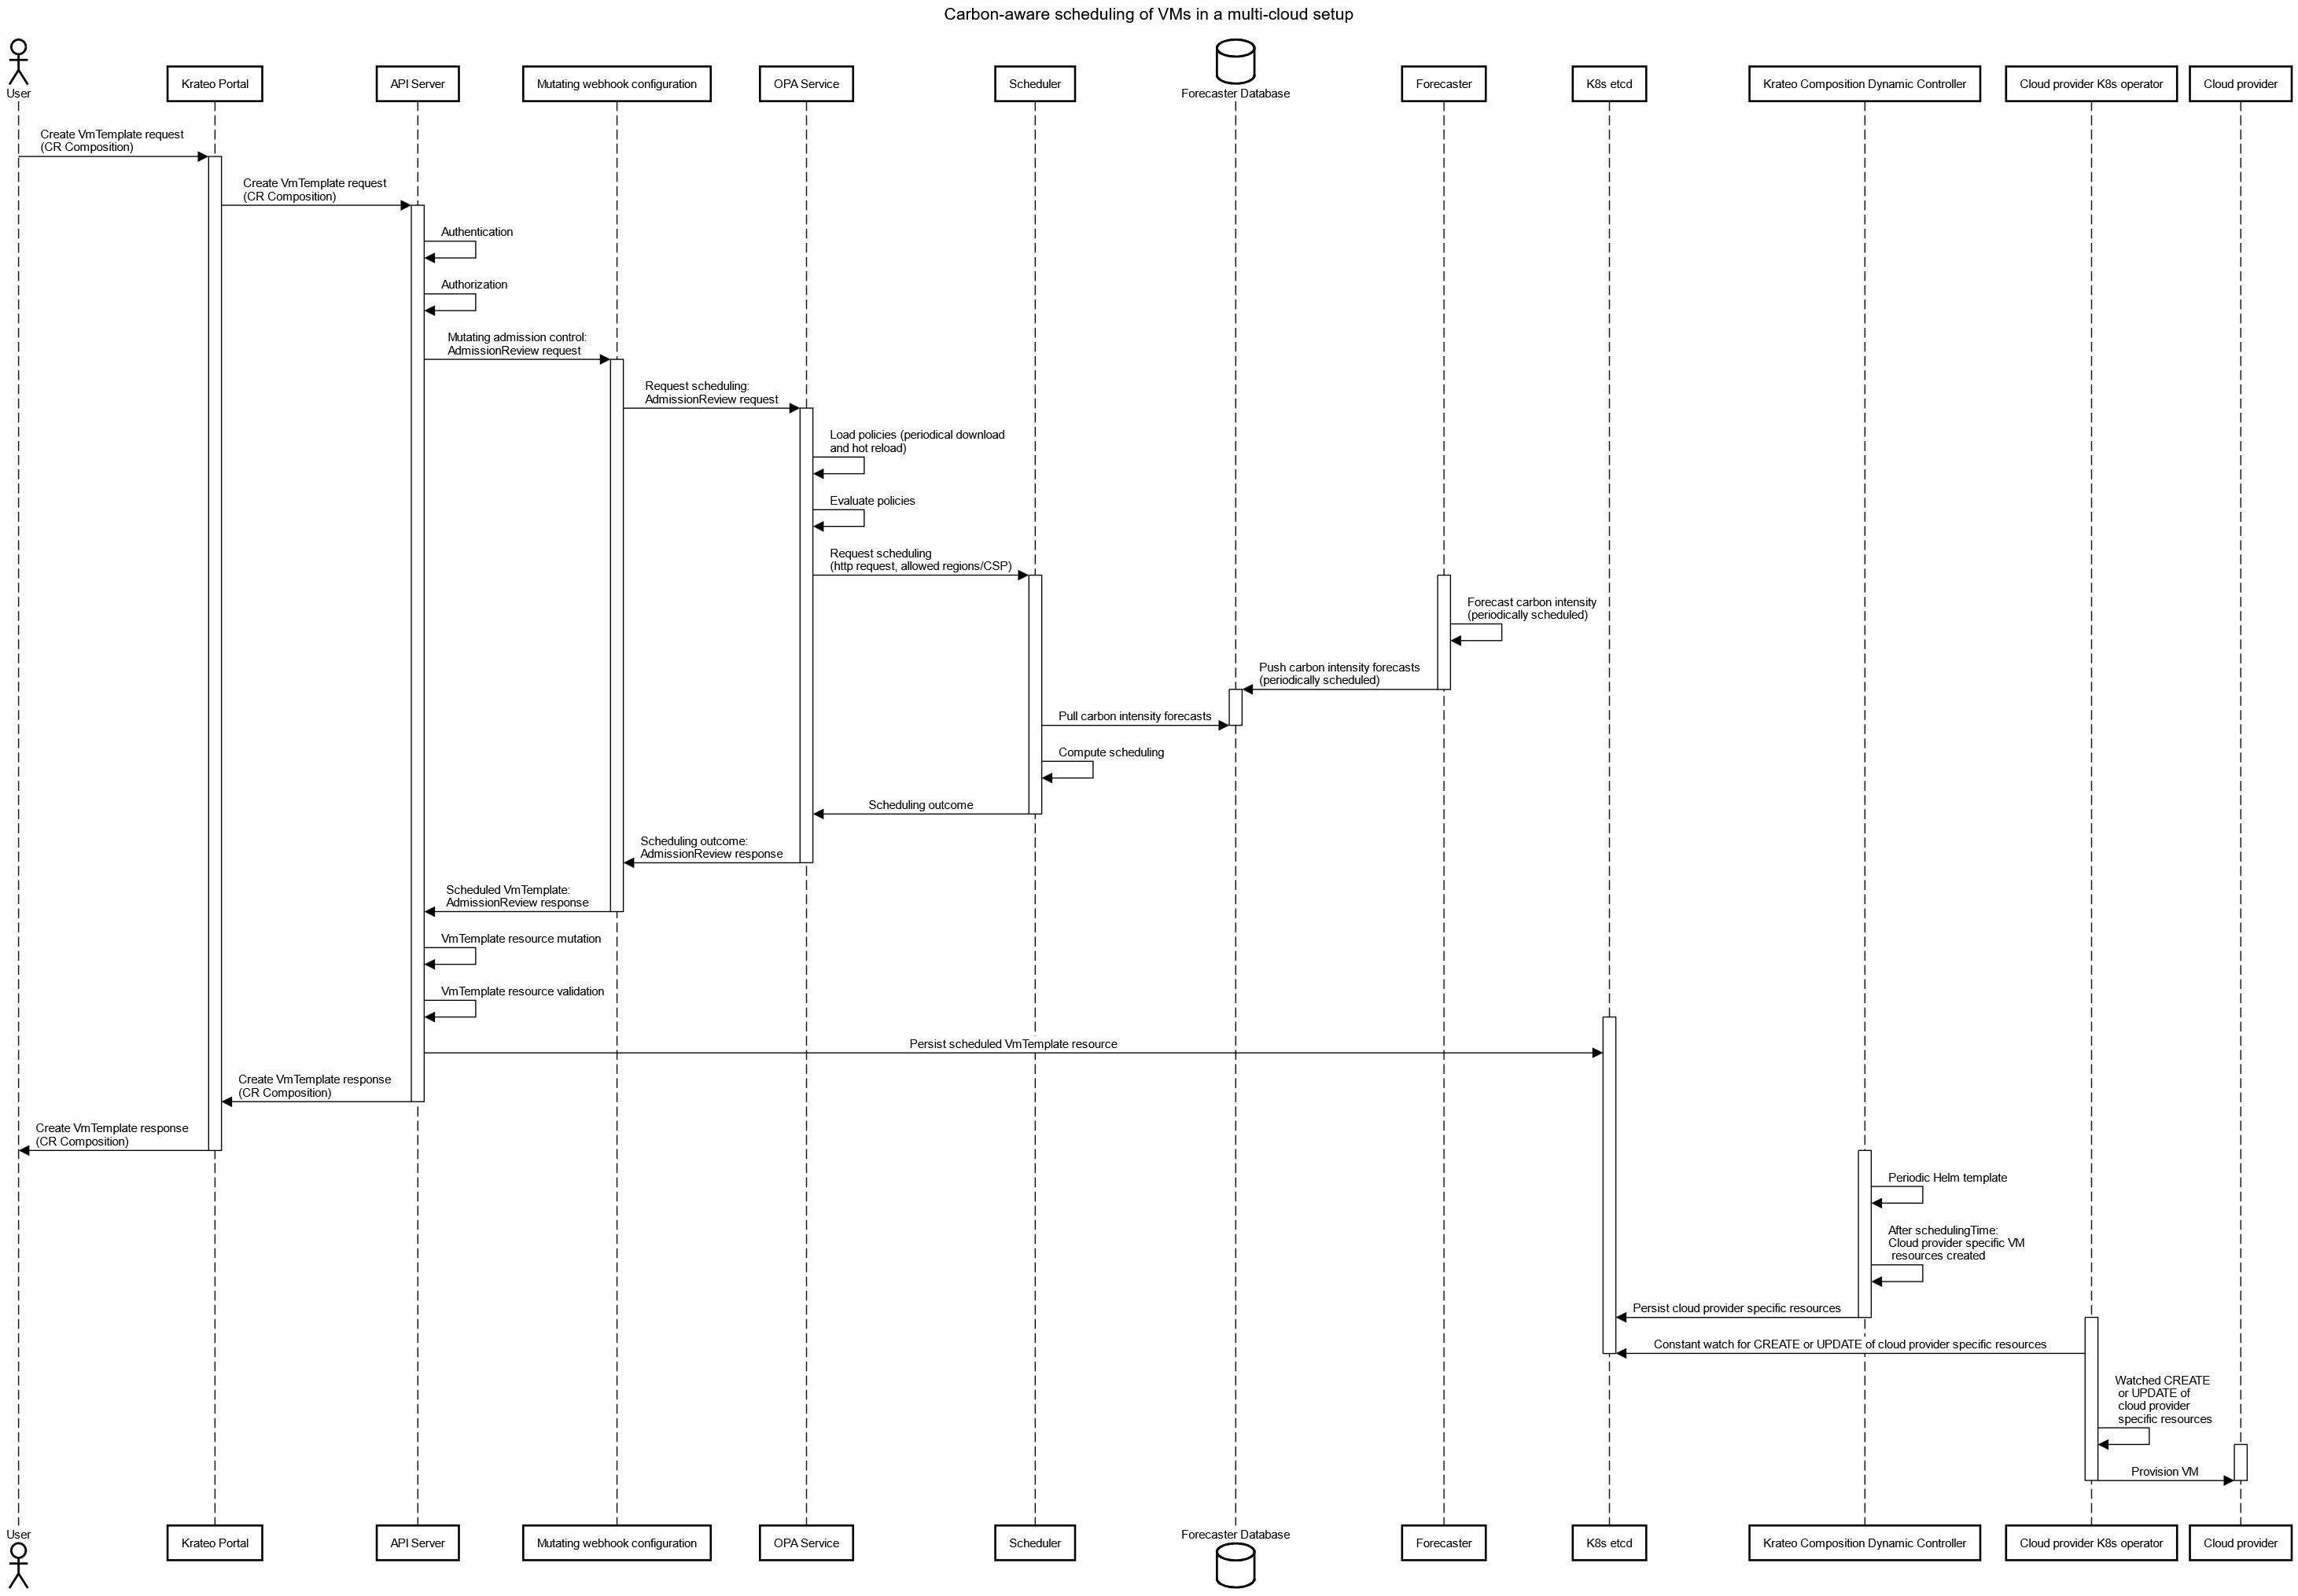
\includegraphics[width=\textheight]{images/sequence_diagram.png}
  \caption{Example of a full-page rotated image}
  \label{fig:rotated_image}
\end{sidewaysfigure}


\newpage







Table for recap of all tools used

Kubernetes
- Krateo
Helm
    Helm charts
    Helm templating
    Helm lookup function

- VmTemplate Krateo Composition Definition
- Azure K8s Operator
- GCP K8s Operator
- AWS K8s Operator
- K8s mutating webhook configuration
- OPA server
- opa policies
- OPA bundles
- MLflow tracking server (+ metadata store & artifact store)
- Forecaster (deployed as KServe InferenceService)


\newpage
